
\appendix
\section{Engineering Drawings} \label{App:AppendixA}

\begin{figure} [H]
\centering
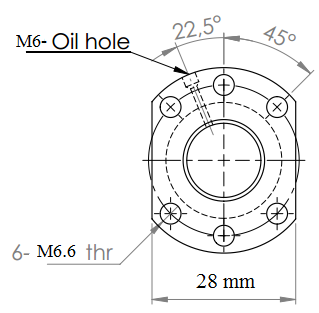
\includegraphics[width=0.6\textwidth]{figures/MechBS1}
\caption{Ball screw nut} \cite{aluflex}
\label{fig:MechBS1}
\end{figure}

\begin{figure} [H]
\centering
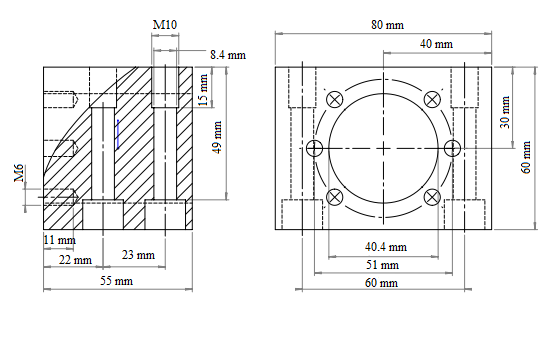
\includegraphics[width=0.8\textwidth]{figures/MechBS3}
\caption{Ball screw nut bracket MGD25} \cite{aluflex}
\label{fig:MechBS2}
\end{figure}


\begin{figure} [H]
\centering
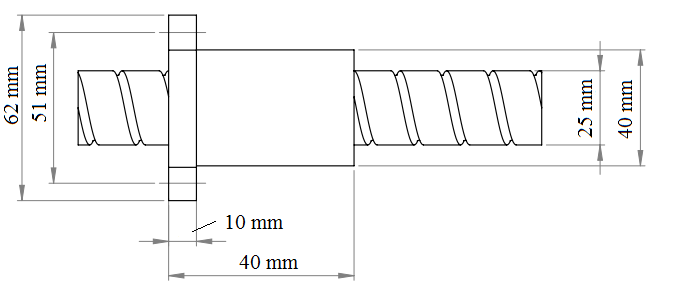
\includegraphics[width=0.8\textwidth]{figures/MechBS2}
\caption{Ball screw (MBA20-E-Comp)} \cite{aluflex}
\label{fig:MechBS2}
\end{figure}


\begin{figure} [H]
\centering
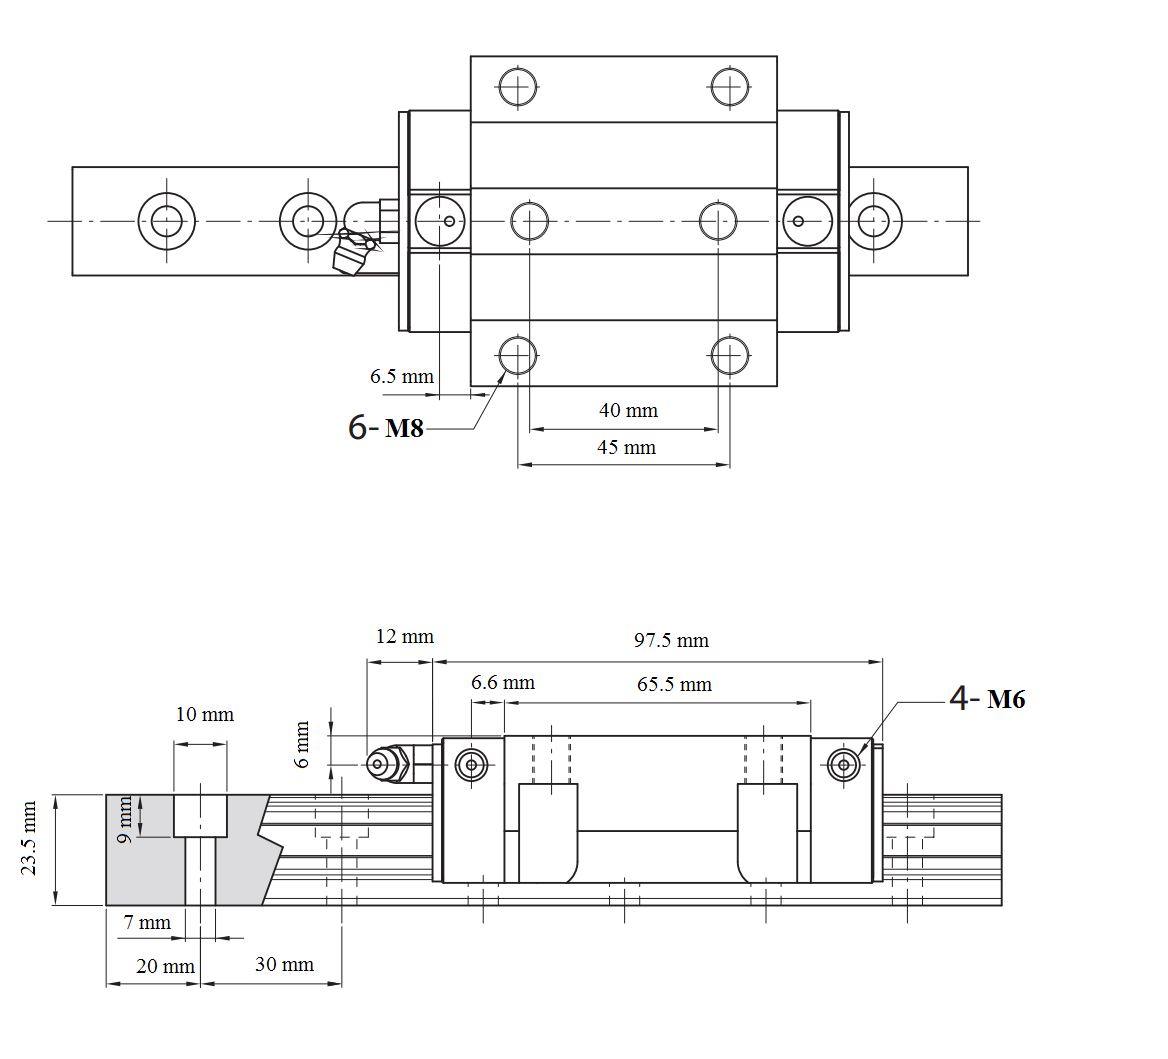
\includegraphics[width=0.8\textwidth]{figures/MechLBG1}
\caption{Complete linear roller guide package (MSR25 E) } \cite{Aluflex_LRG}
\label{fig:MechLRG1}
\end{figure}



\begin{figure} [H]
\centering
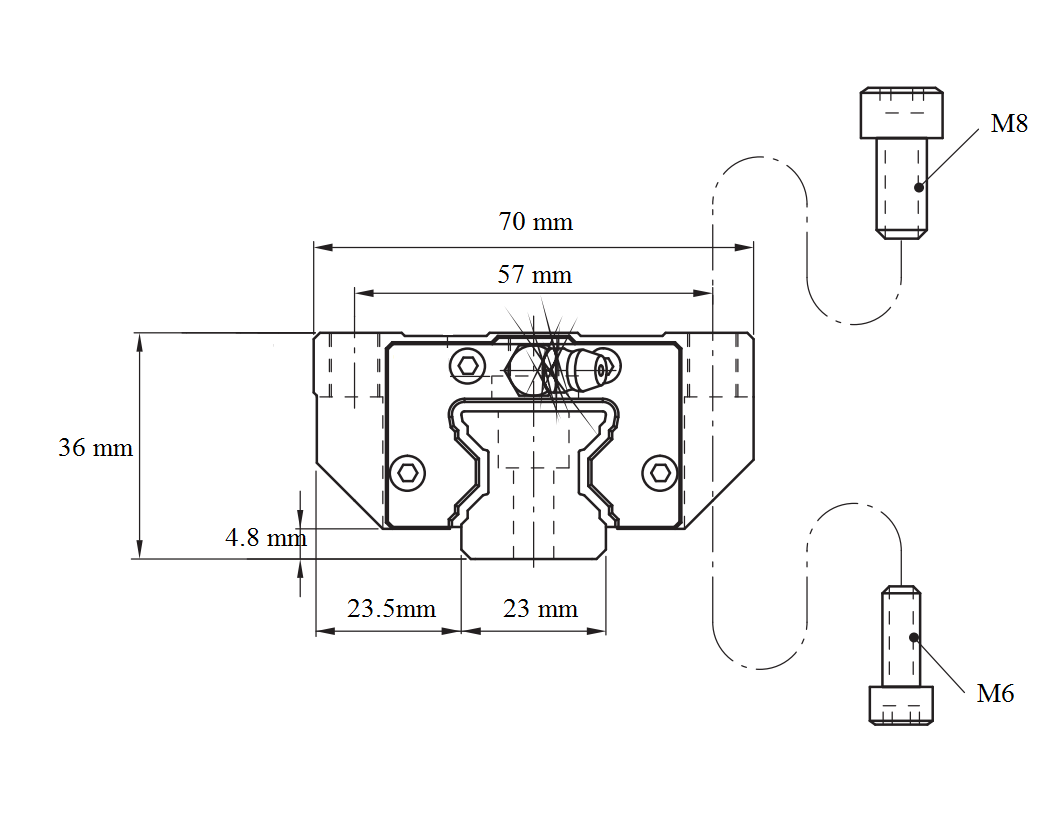
\includegraphics[width=0.8\textwidth]{figures/MechLBG2}
\caption{Linear roller guide carriage} \cite{Aluflex_LRG}
\label{fig:MechLRG2}
\end{figure}

\begin{figure} [H]
\centering
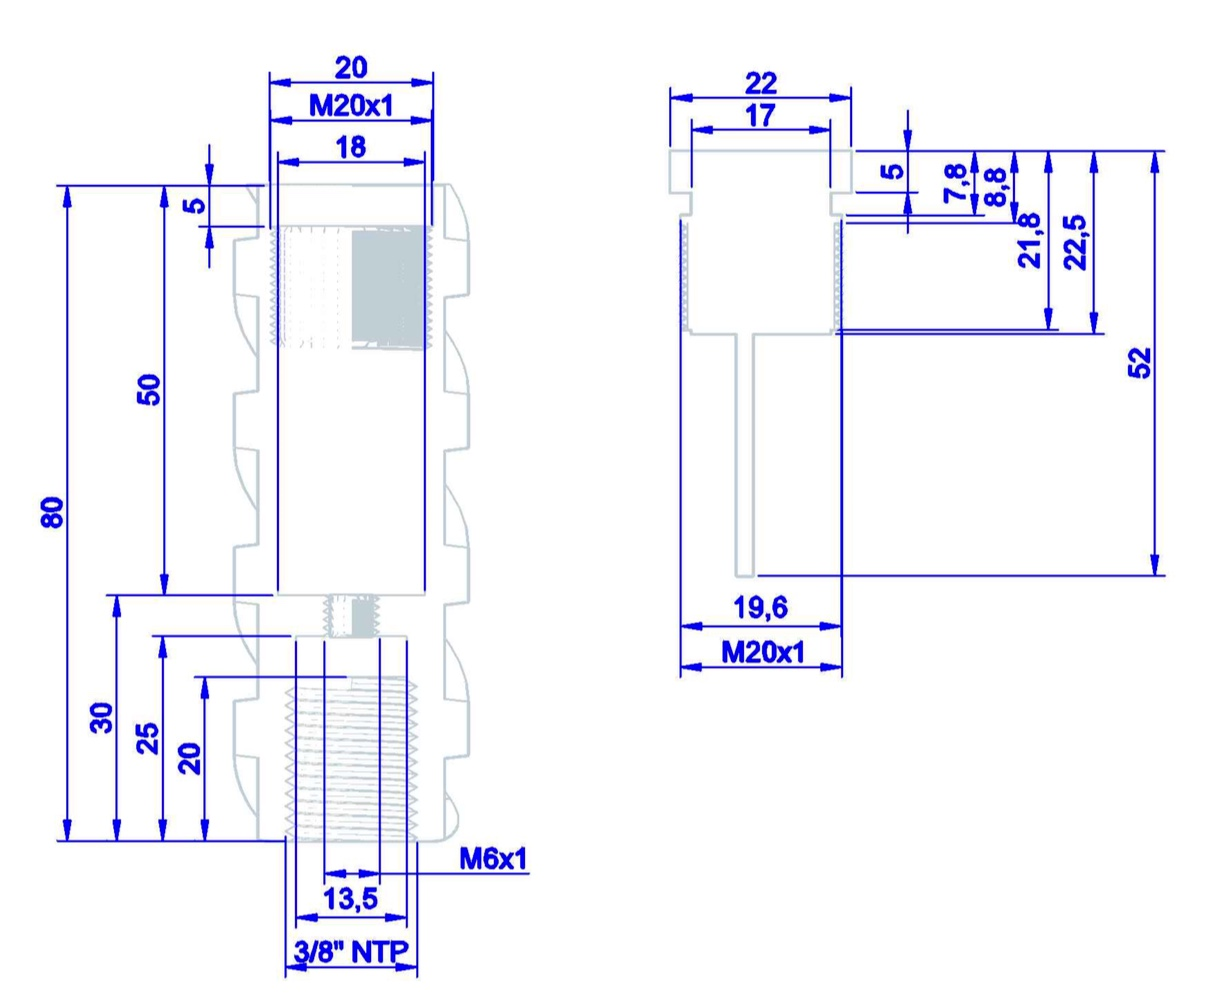
\includegraphics[width=0.8\textwidth]{figures/stabdim}
\caption{Side cut of stabilizer on the left hand side and sensor plate to be placed inside BHA on the right hand side. All dimensions in mm} 
\label{fig:StabDim}
\end{figure}

\newpage
\begin{figure} [H]
\centering
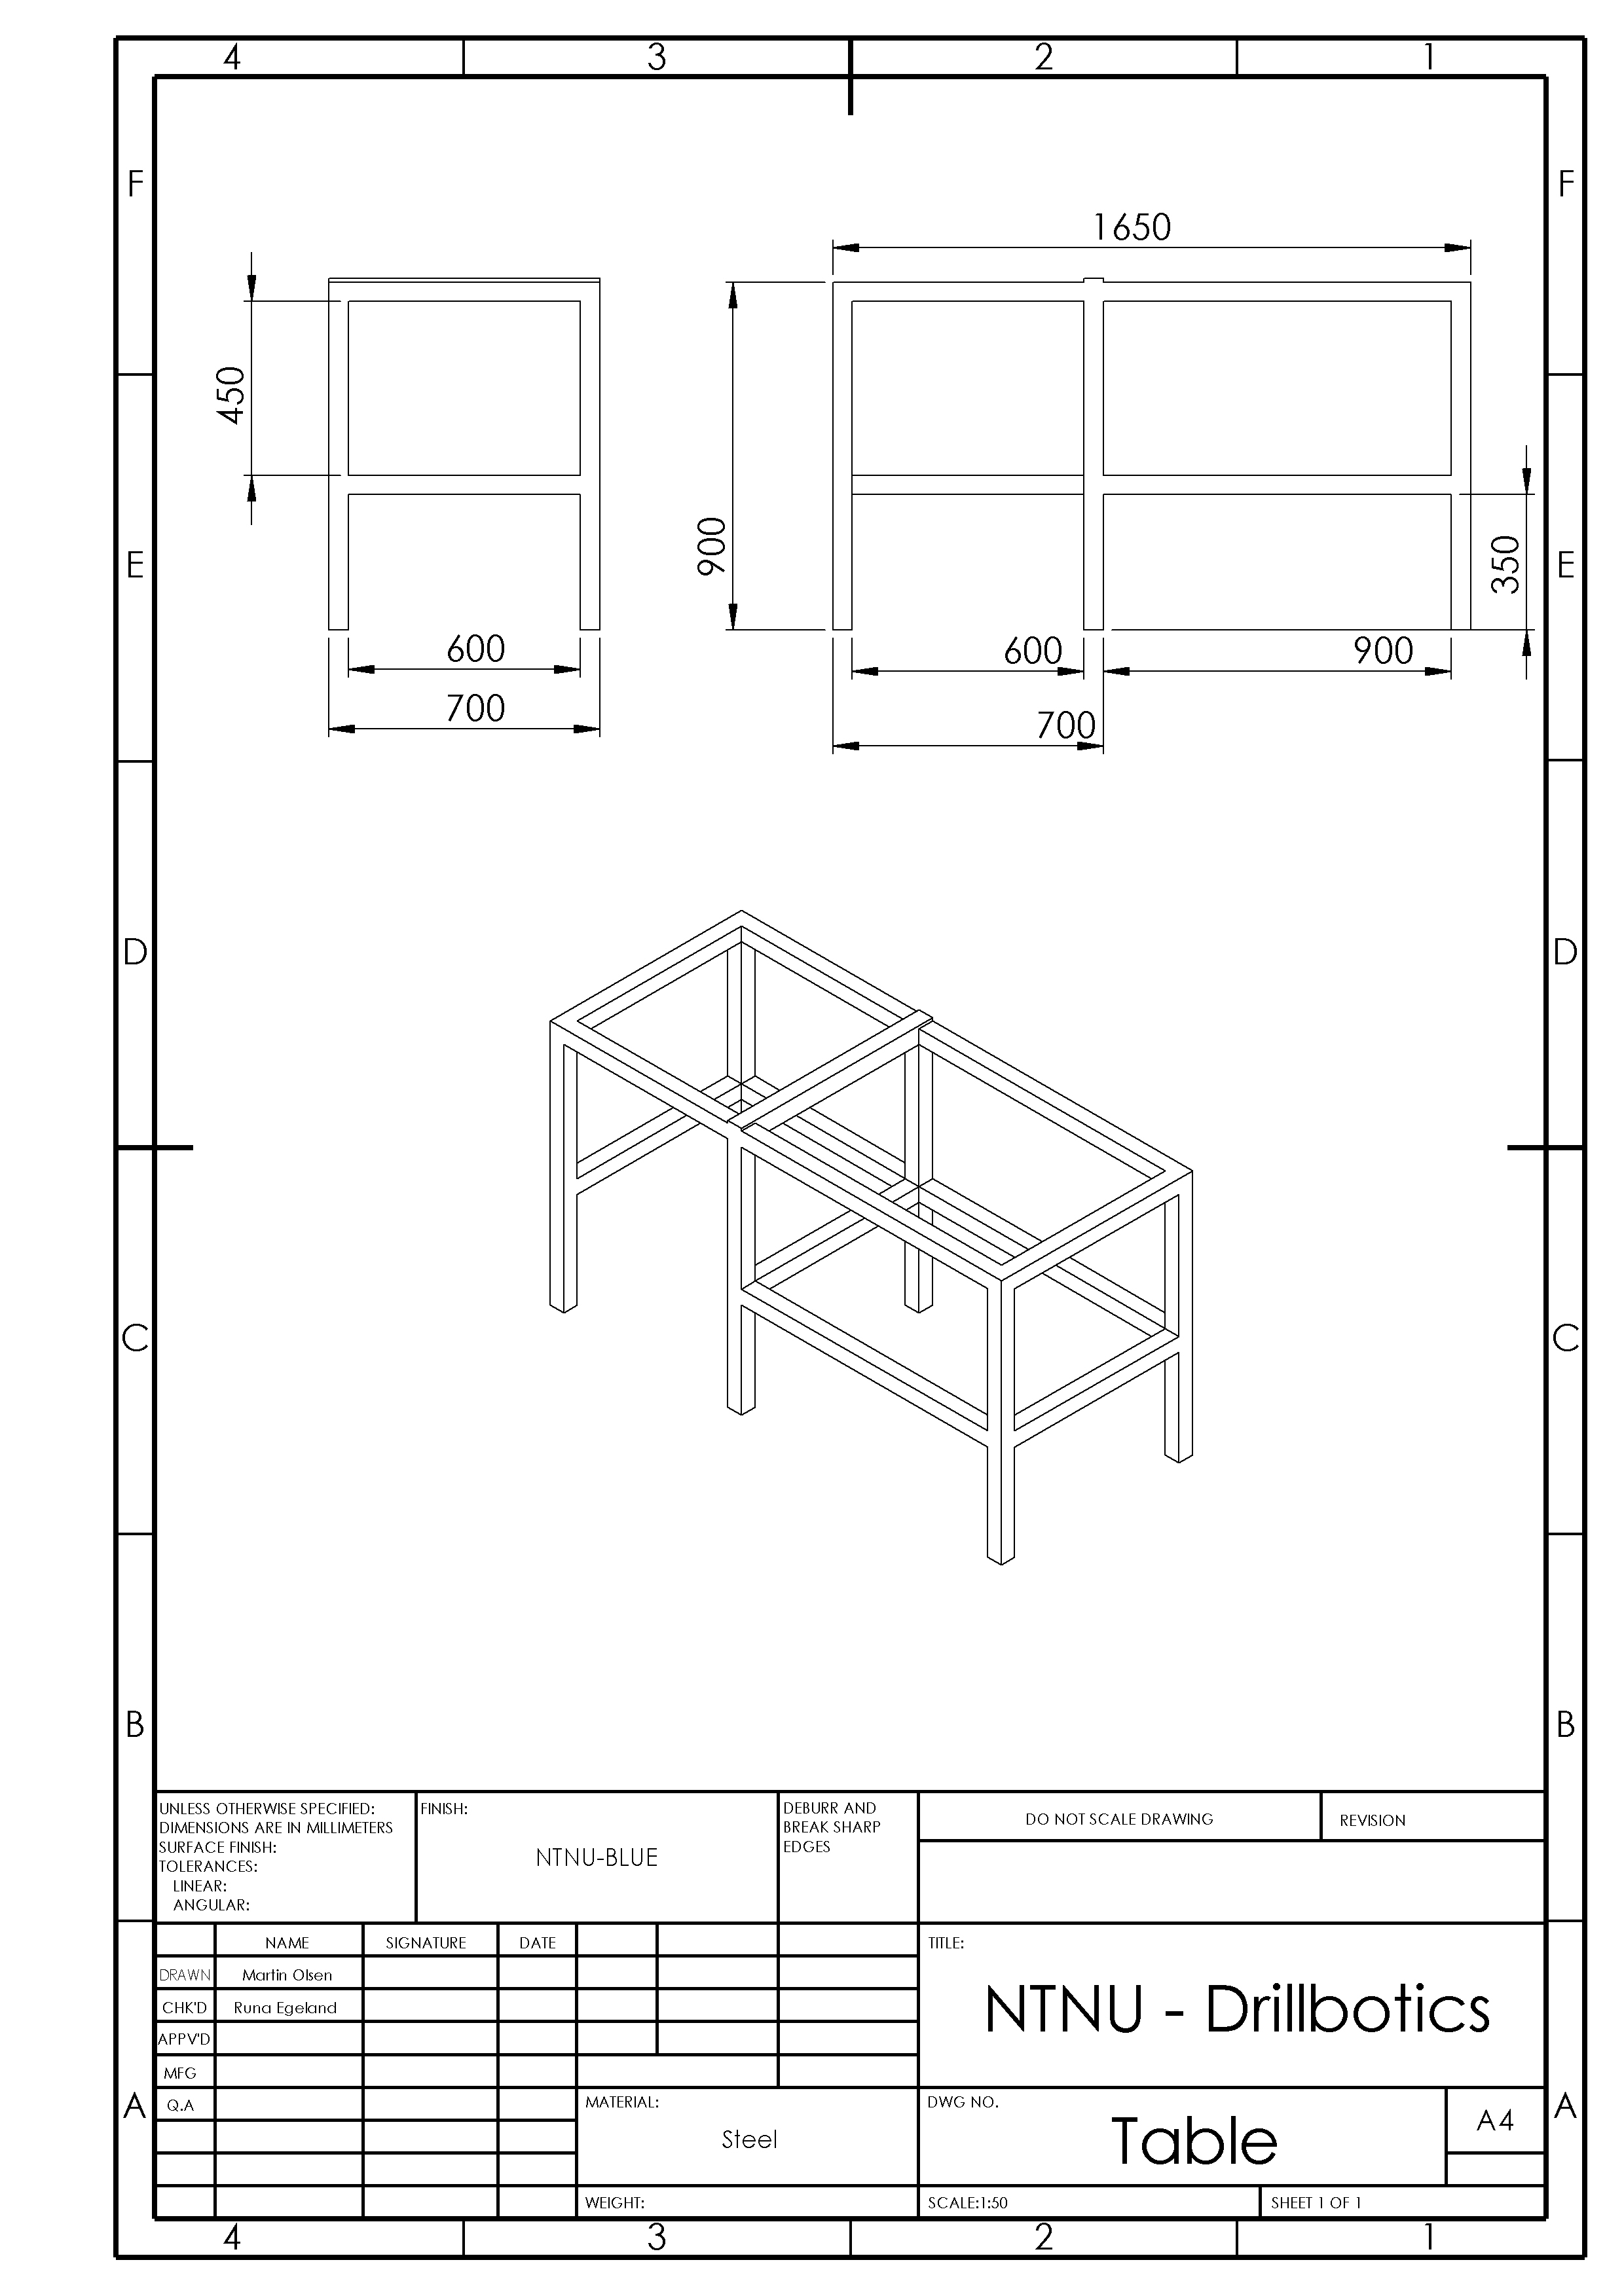
\includegraphics[width=1.0\textwidth]{figures/mechdrawings/Table.JPG}
\caption{Substructure of Rig. All dimensions in mm} 
\label{fig:table}
\end{figure}

\newpage
\begin{figure} [H]
\centering
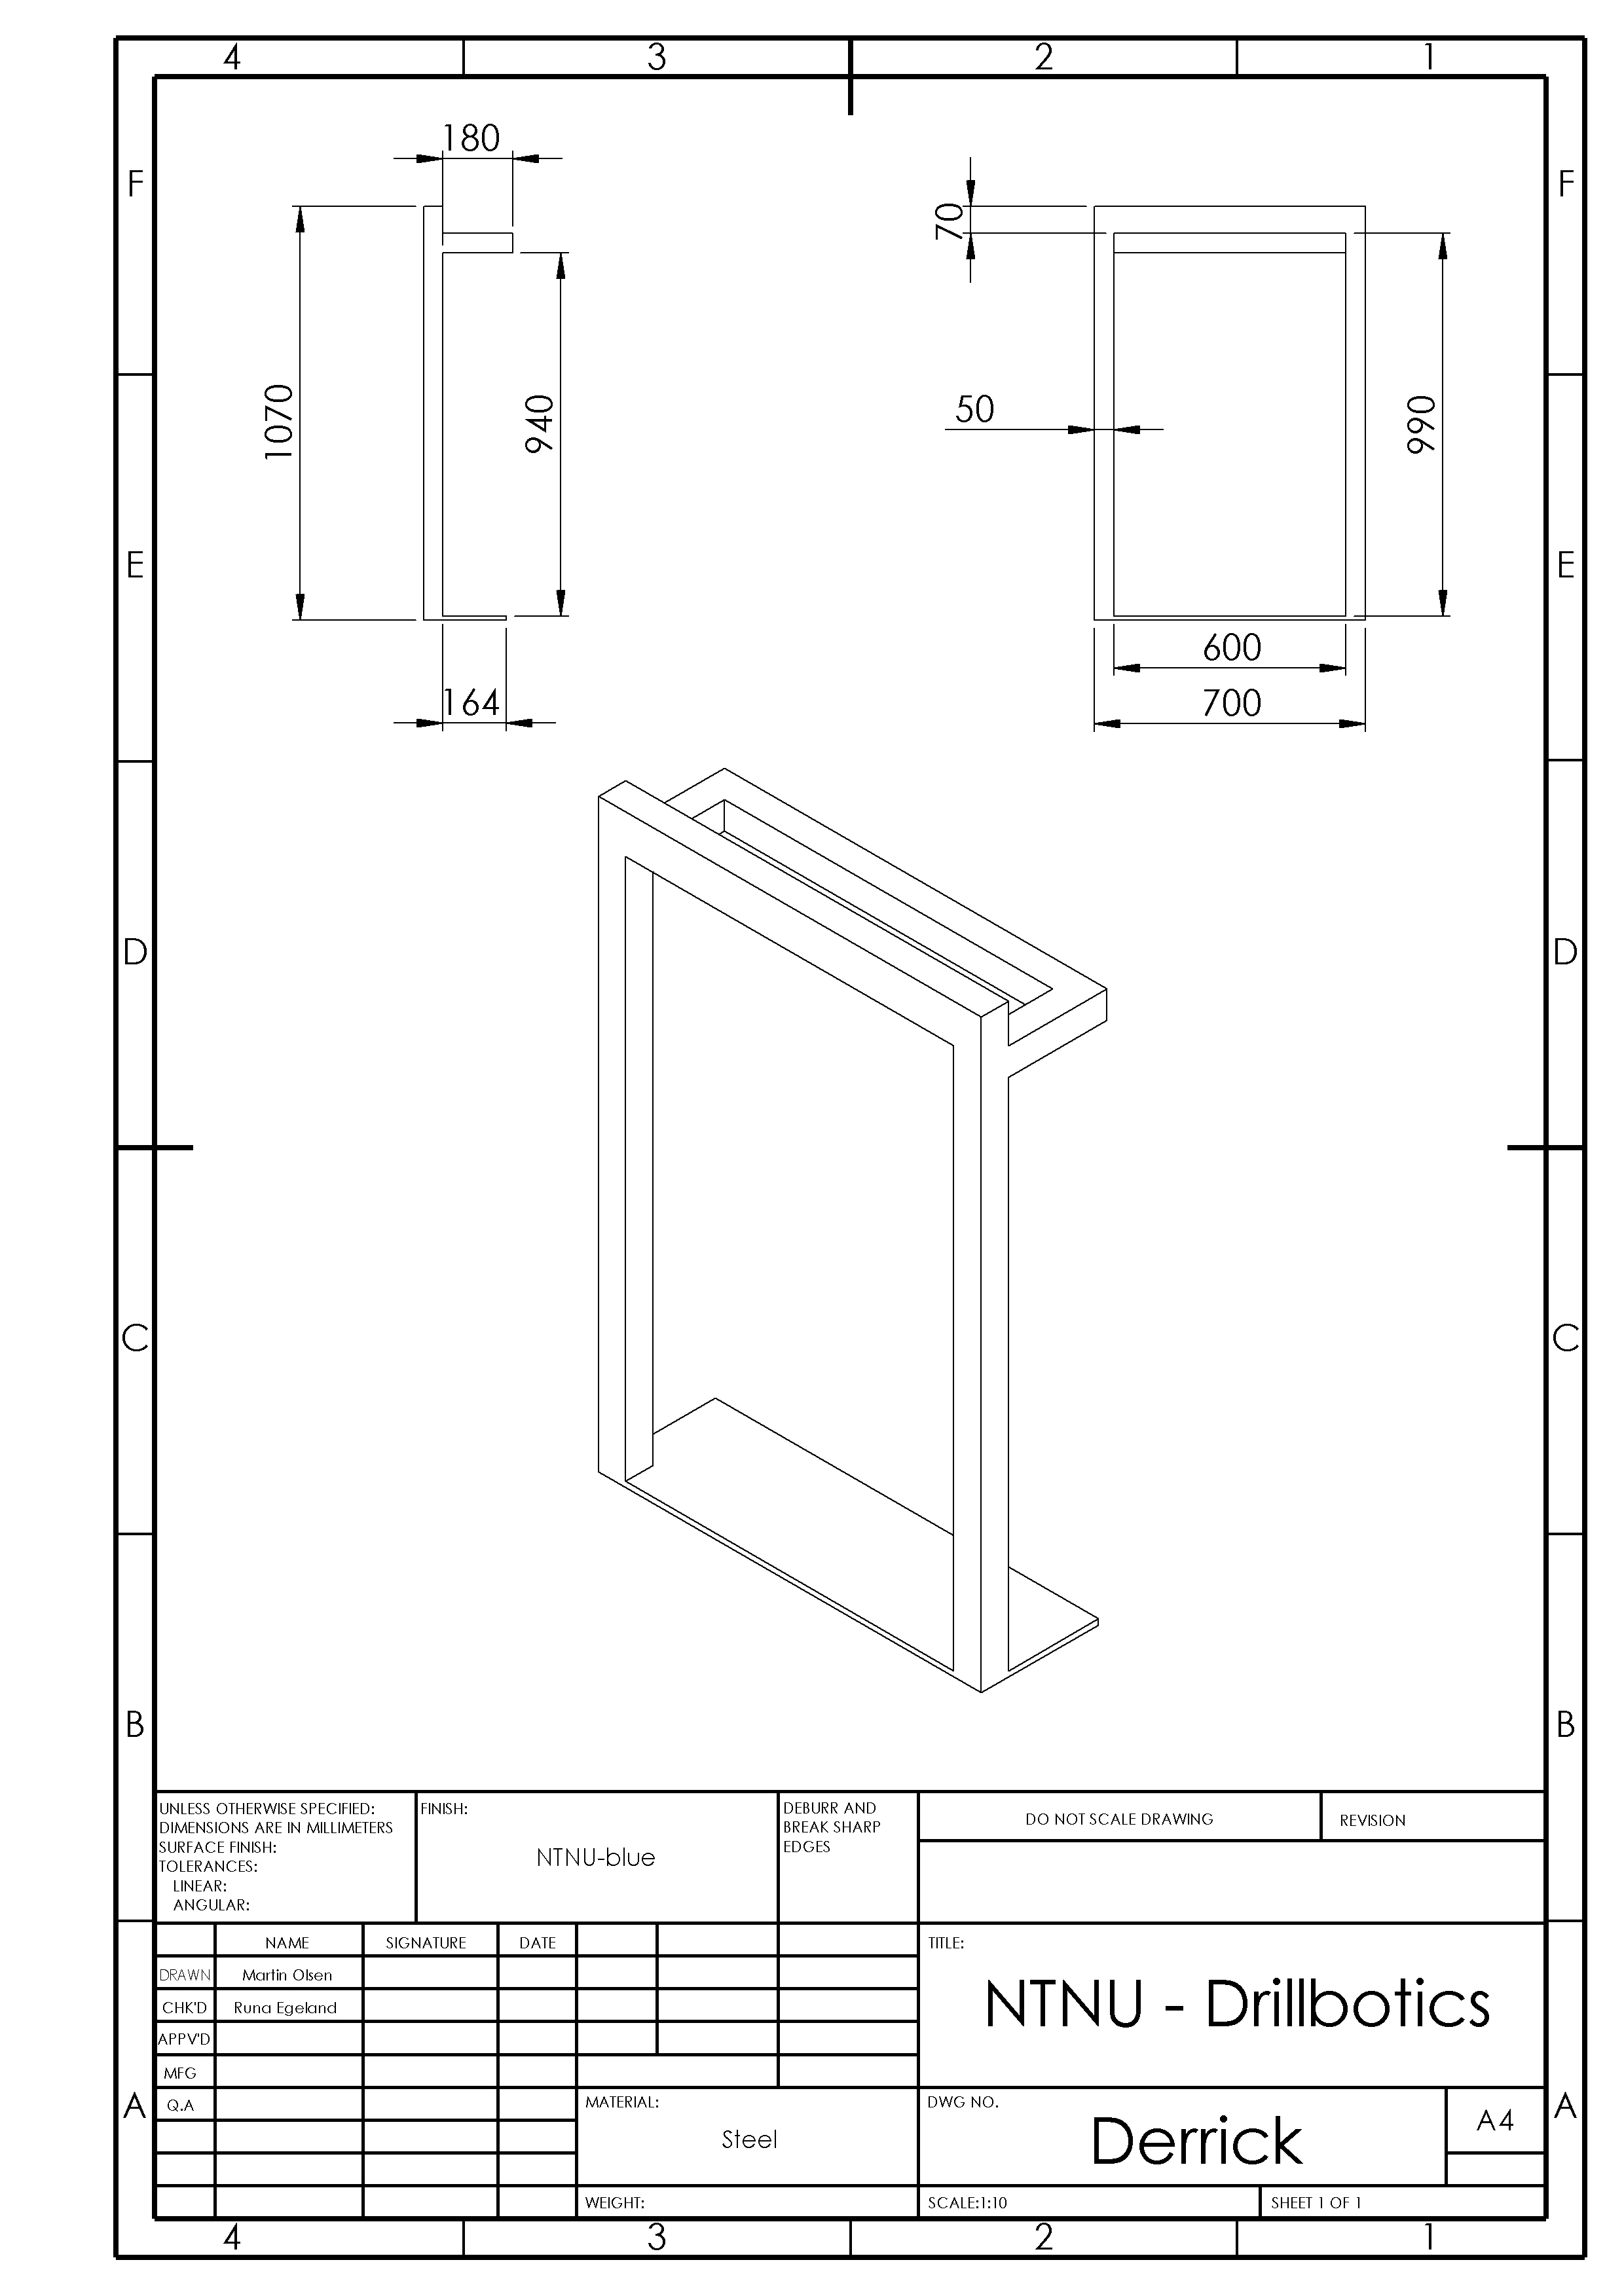
\includegraphics[width=1.0\textwidth]{figures/mechdrawings/Derrick.JPG}
\caption{Derrick. All dimensions in mm} 
\label{fig:Derrick}
\end{figure}

\newpage
\begin{figure} [H]
\centering
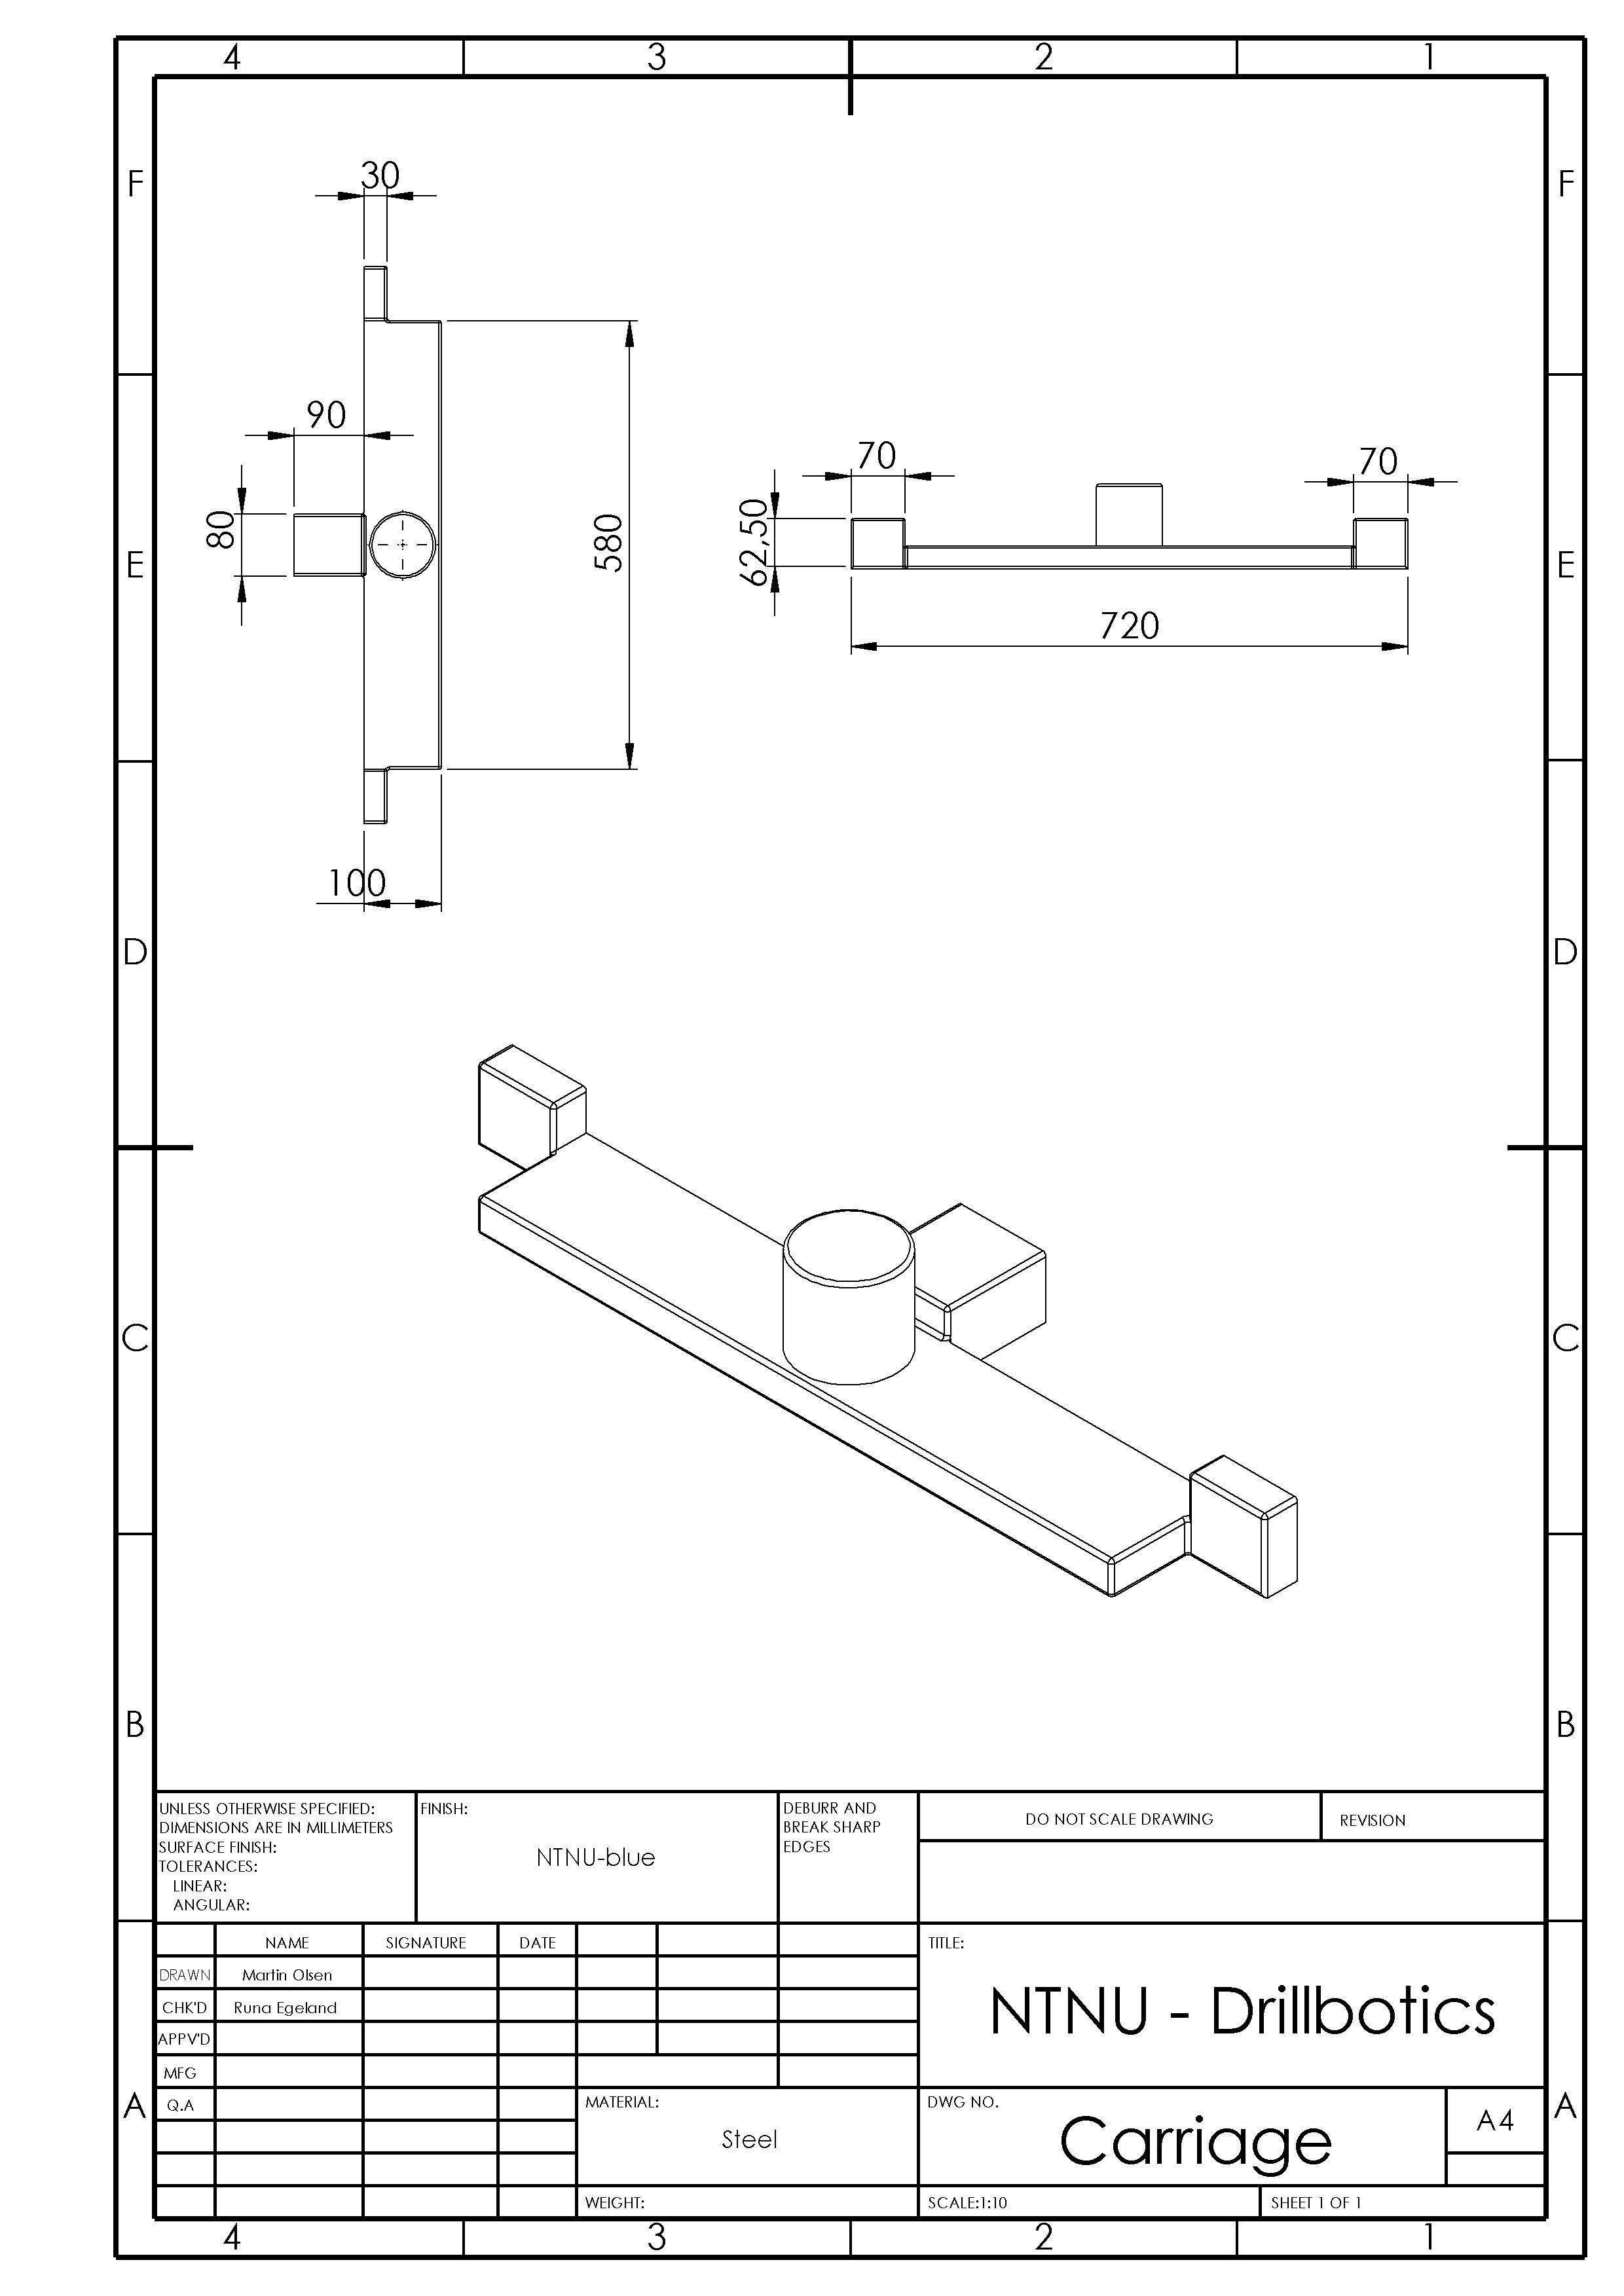
\includegraphics[width=1.0\textwidth]{figures/mechdrawings/Carriage.JPG}
\caption{Carriage. All dimensions in mm} 
\label{fig:Carriage}
\end{figure}

\newpage
\begin{figure} [H]
\centering
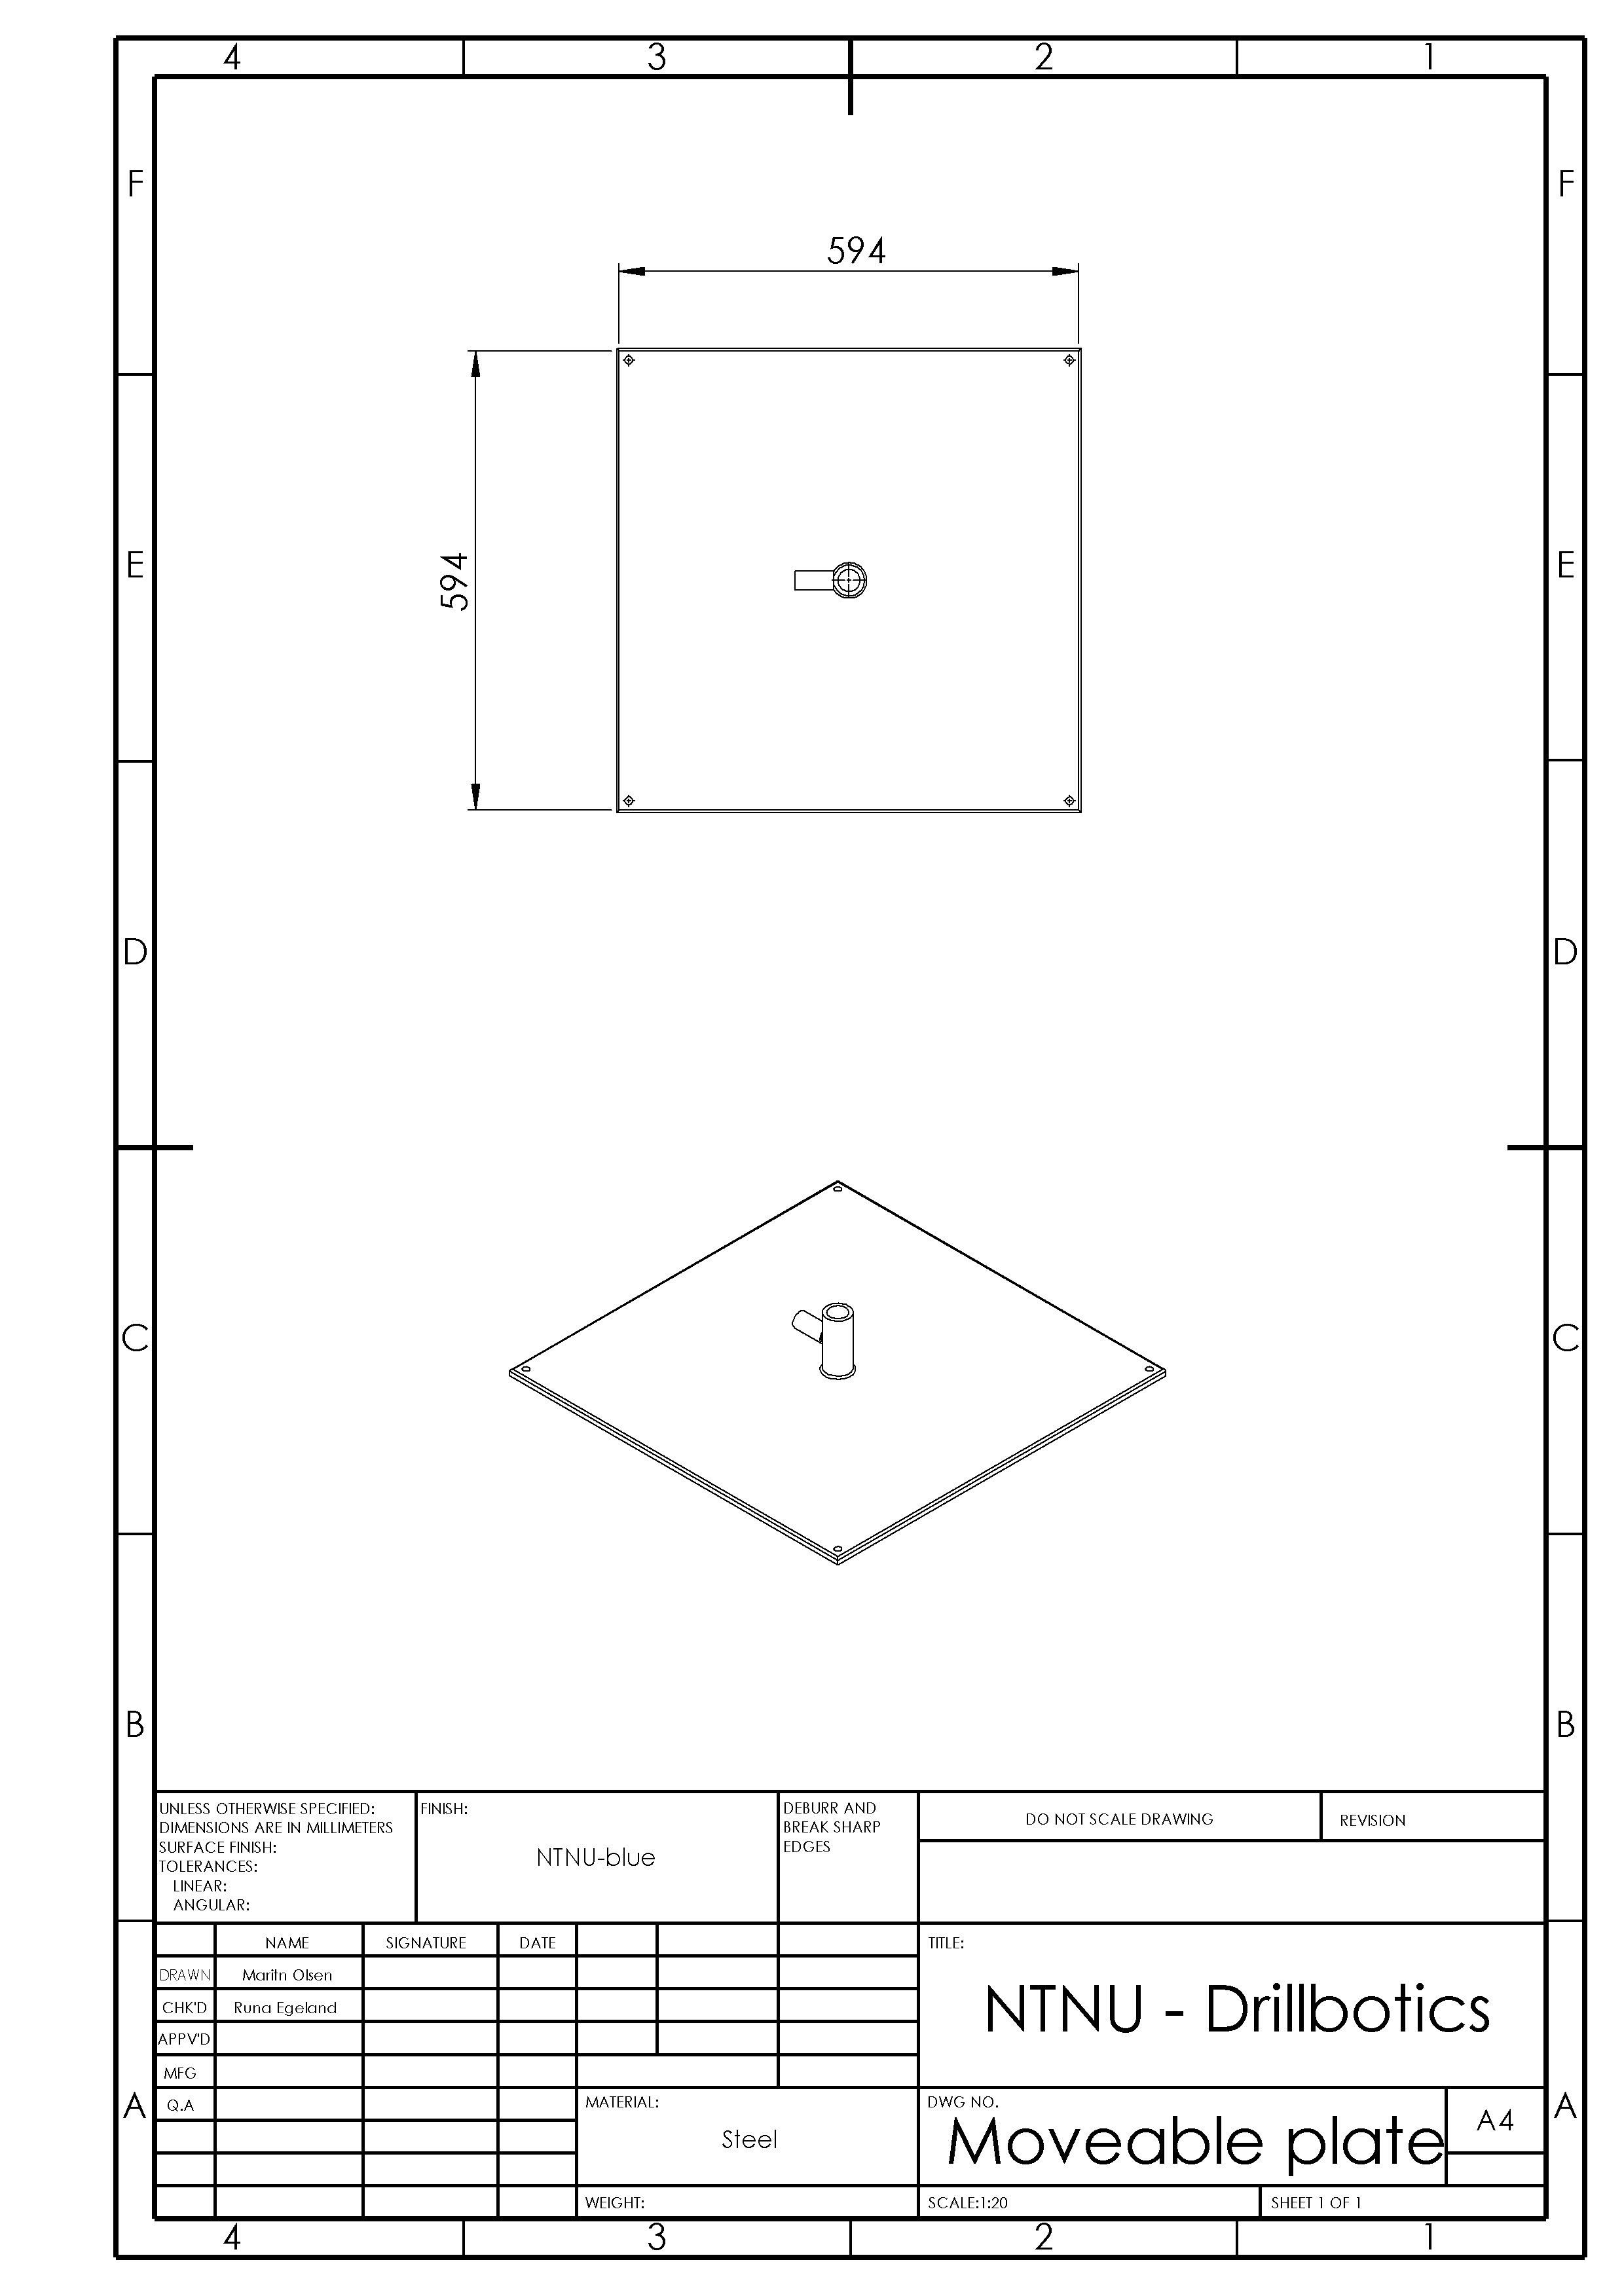
\includegraphics[width=1.0\textwidth]{figures/mechdrawings/Moveableplate.JPG}
\caption{Moveable Plate with Riser. All dimensions in mm} 
\label{fig:riserplate}
\end{figure}

\newpage
\begin{figure} [H]
\centering
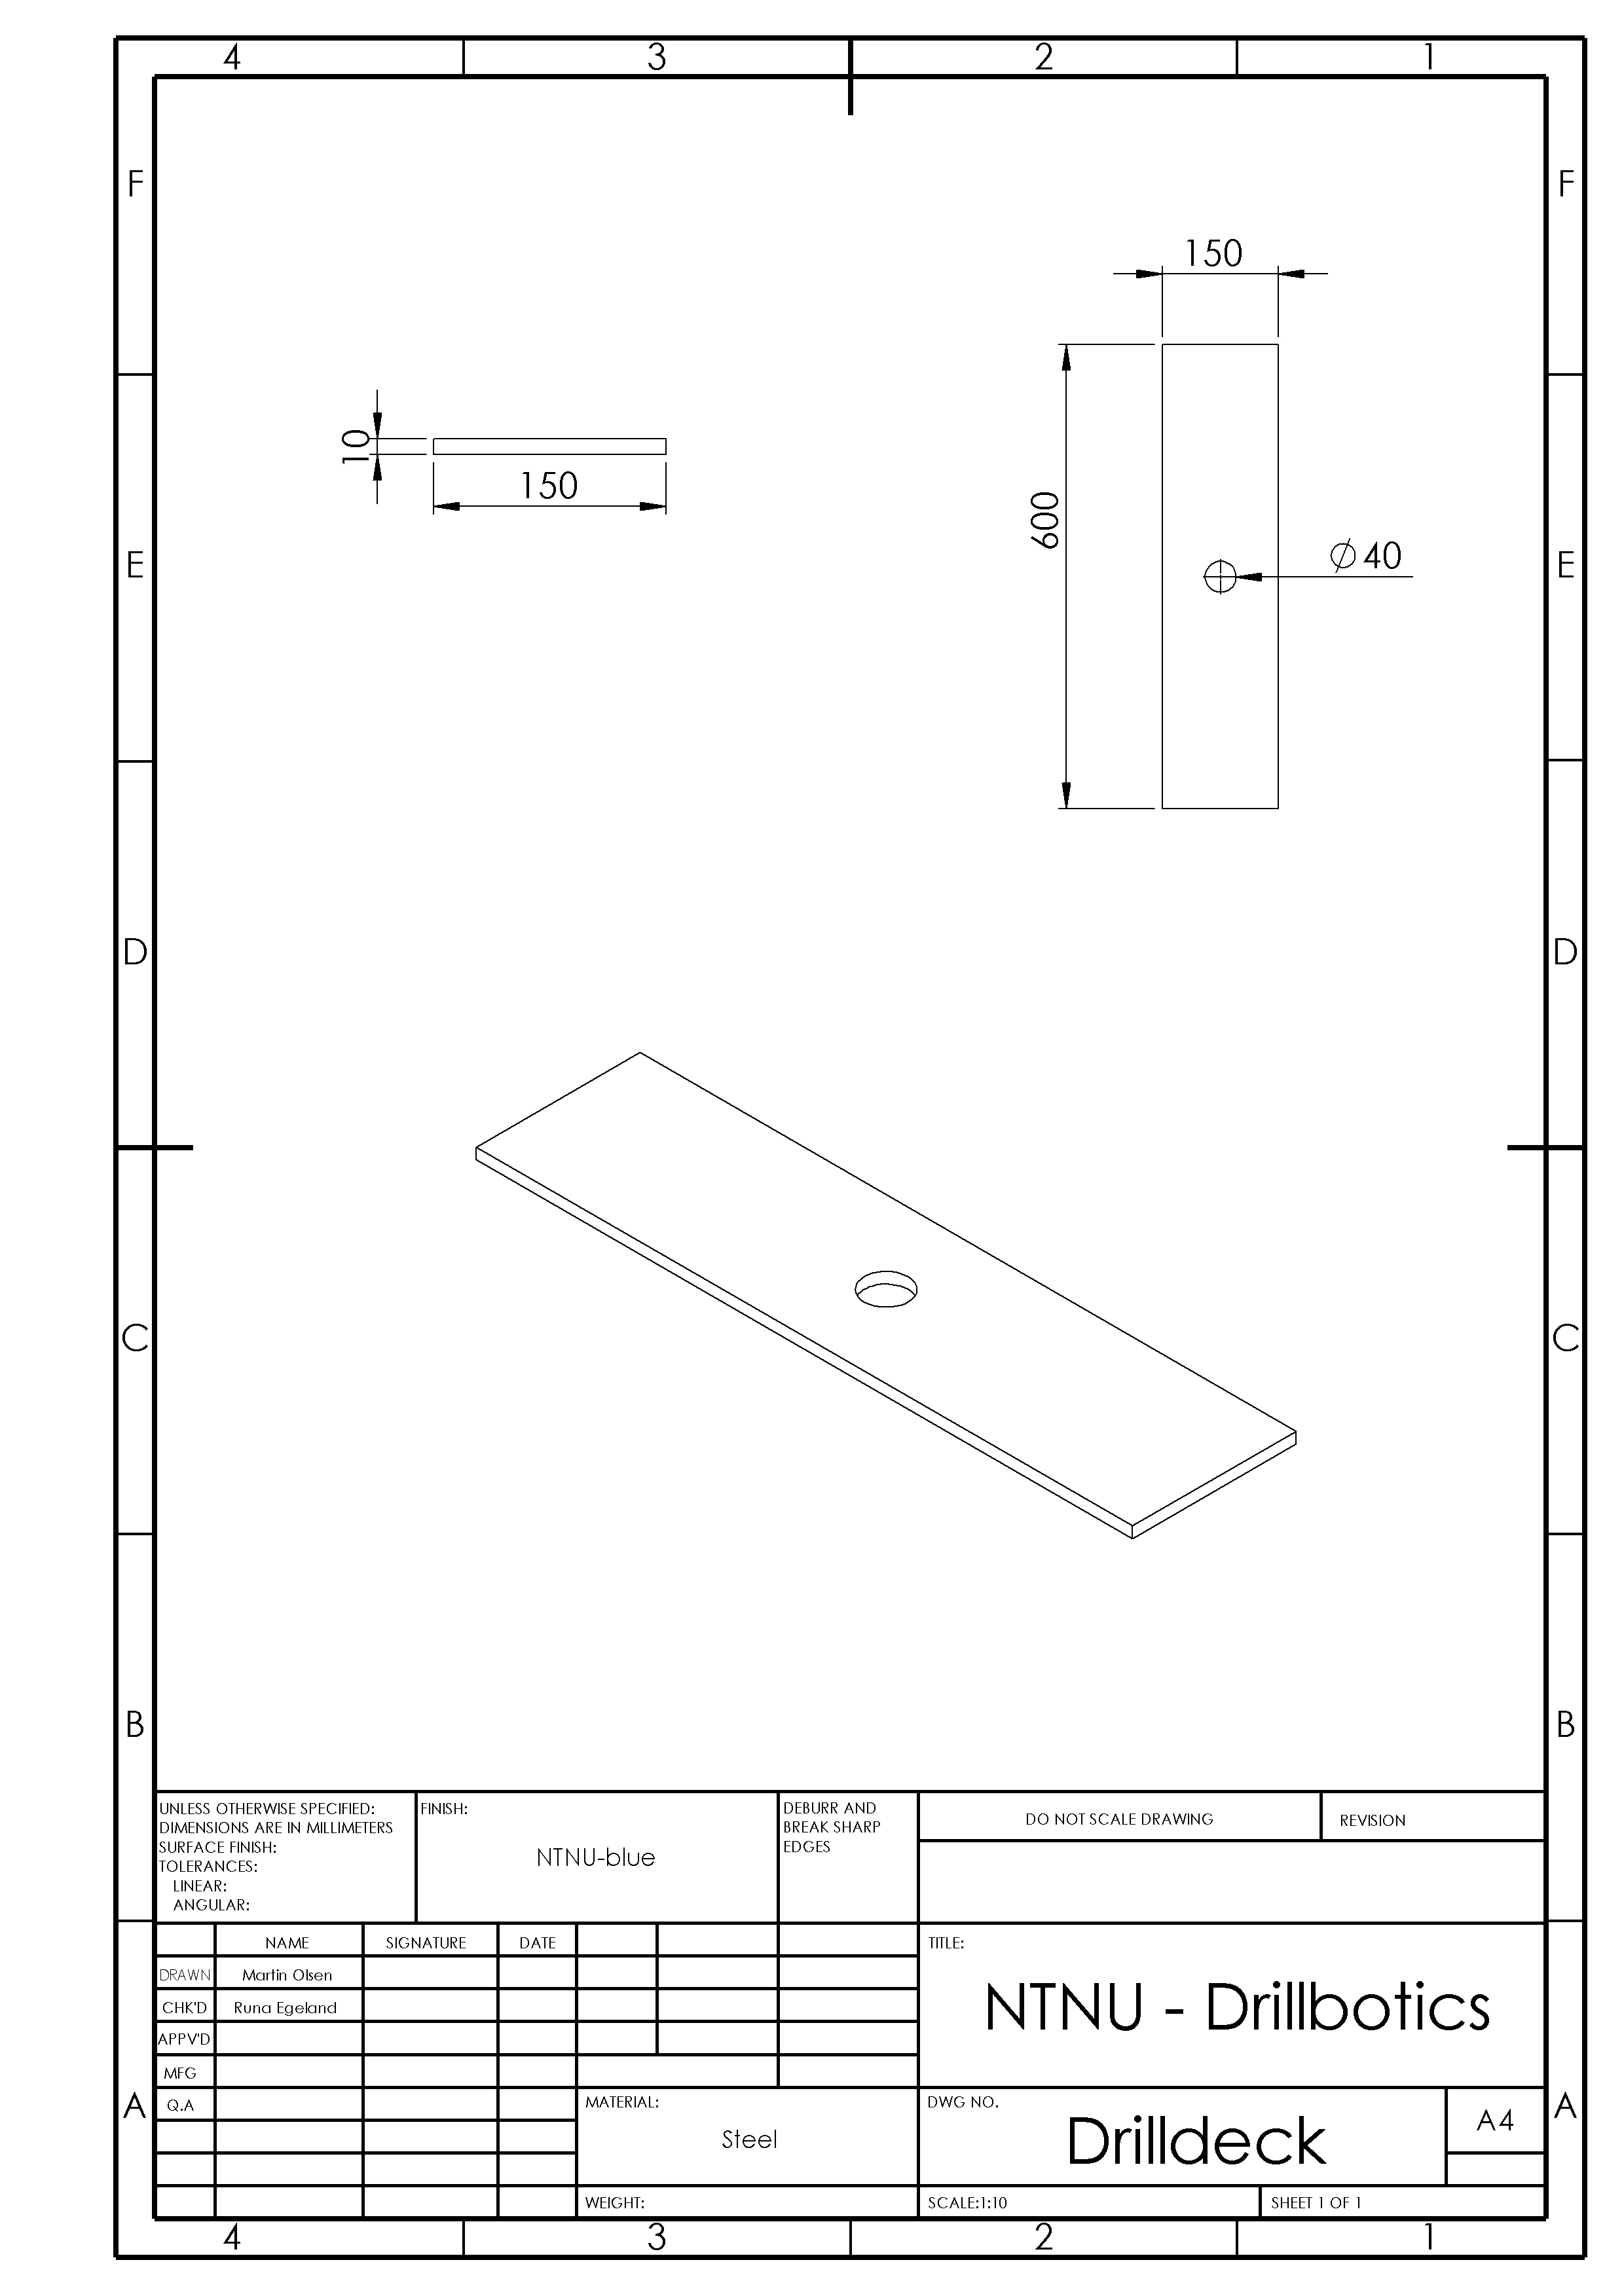
\includegraphics[width=1.0\textwidth]{figures/mechdrawings/Drilldeck.JPG}
\caption{Drilldeck with hole for bushing. All dimensions in mm} 
\label{fig:drilldeck}
\end{figure}

\newpage
\begin{figure} [H]
\centering
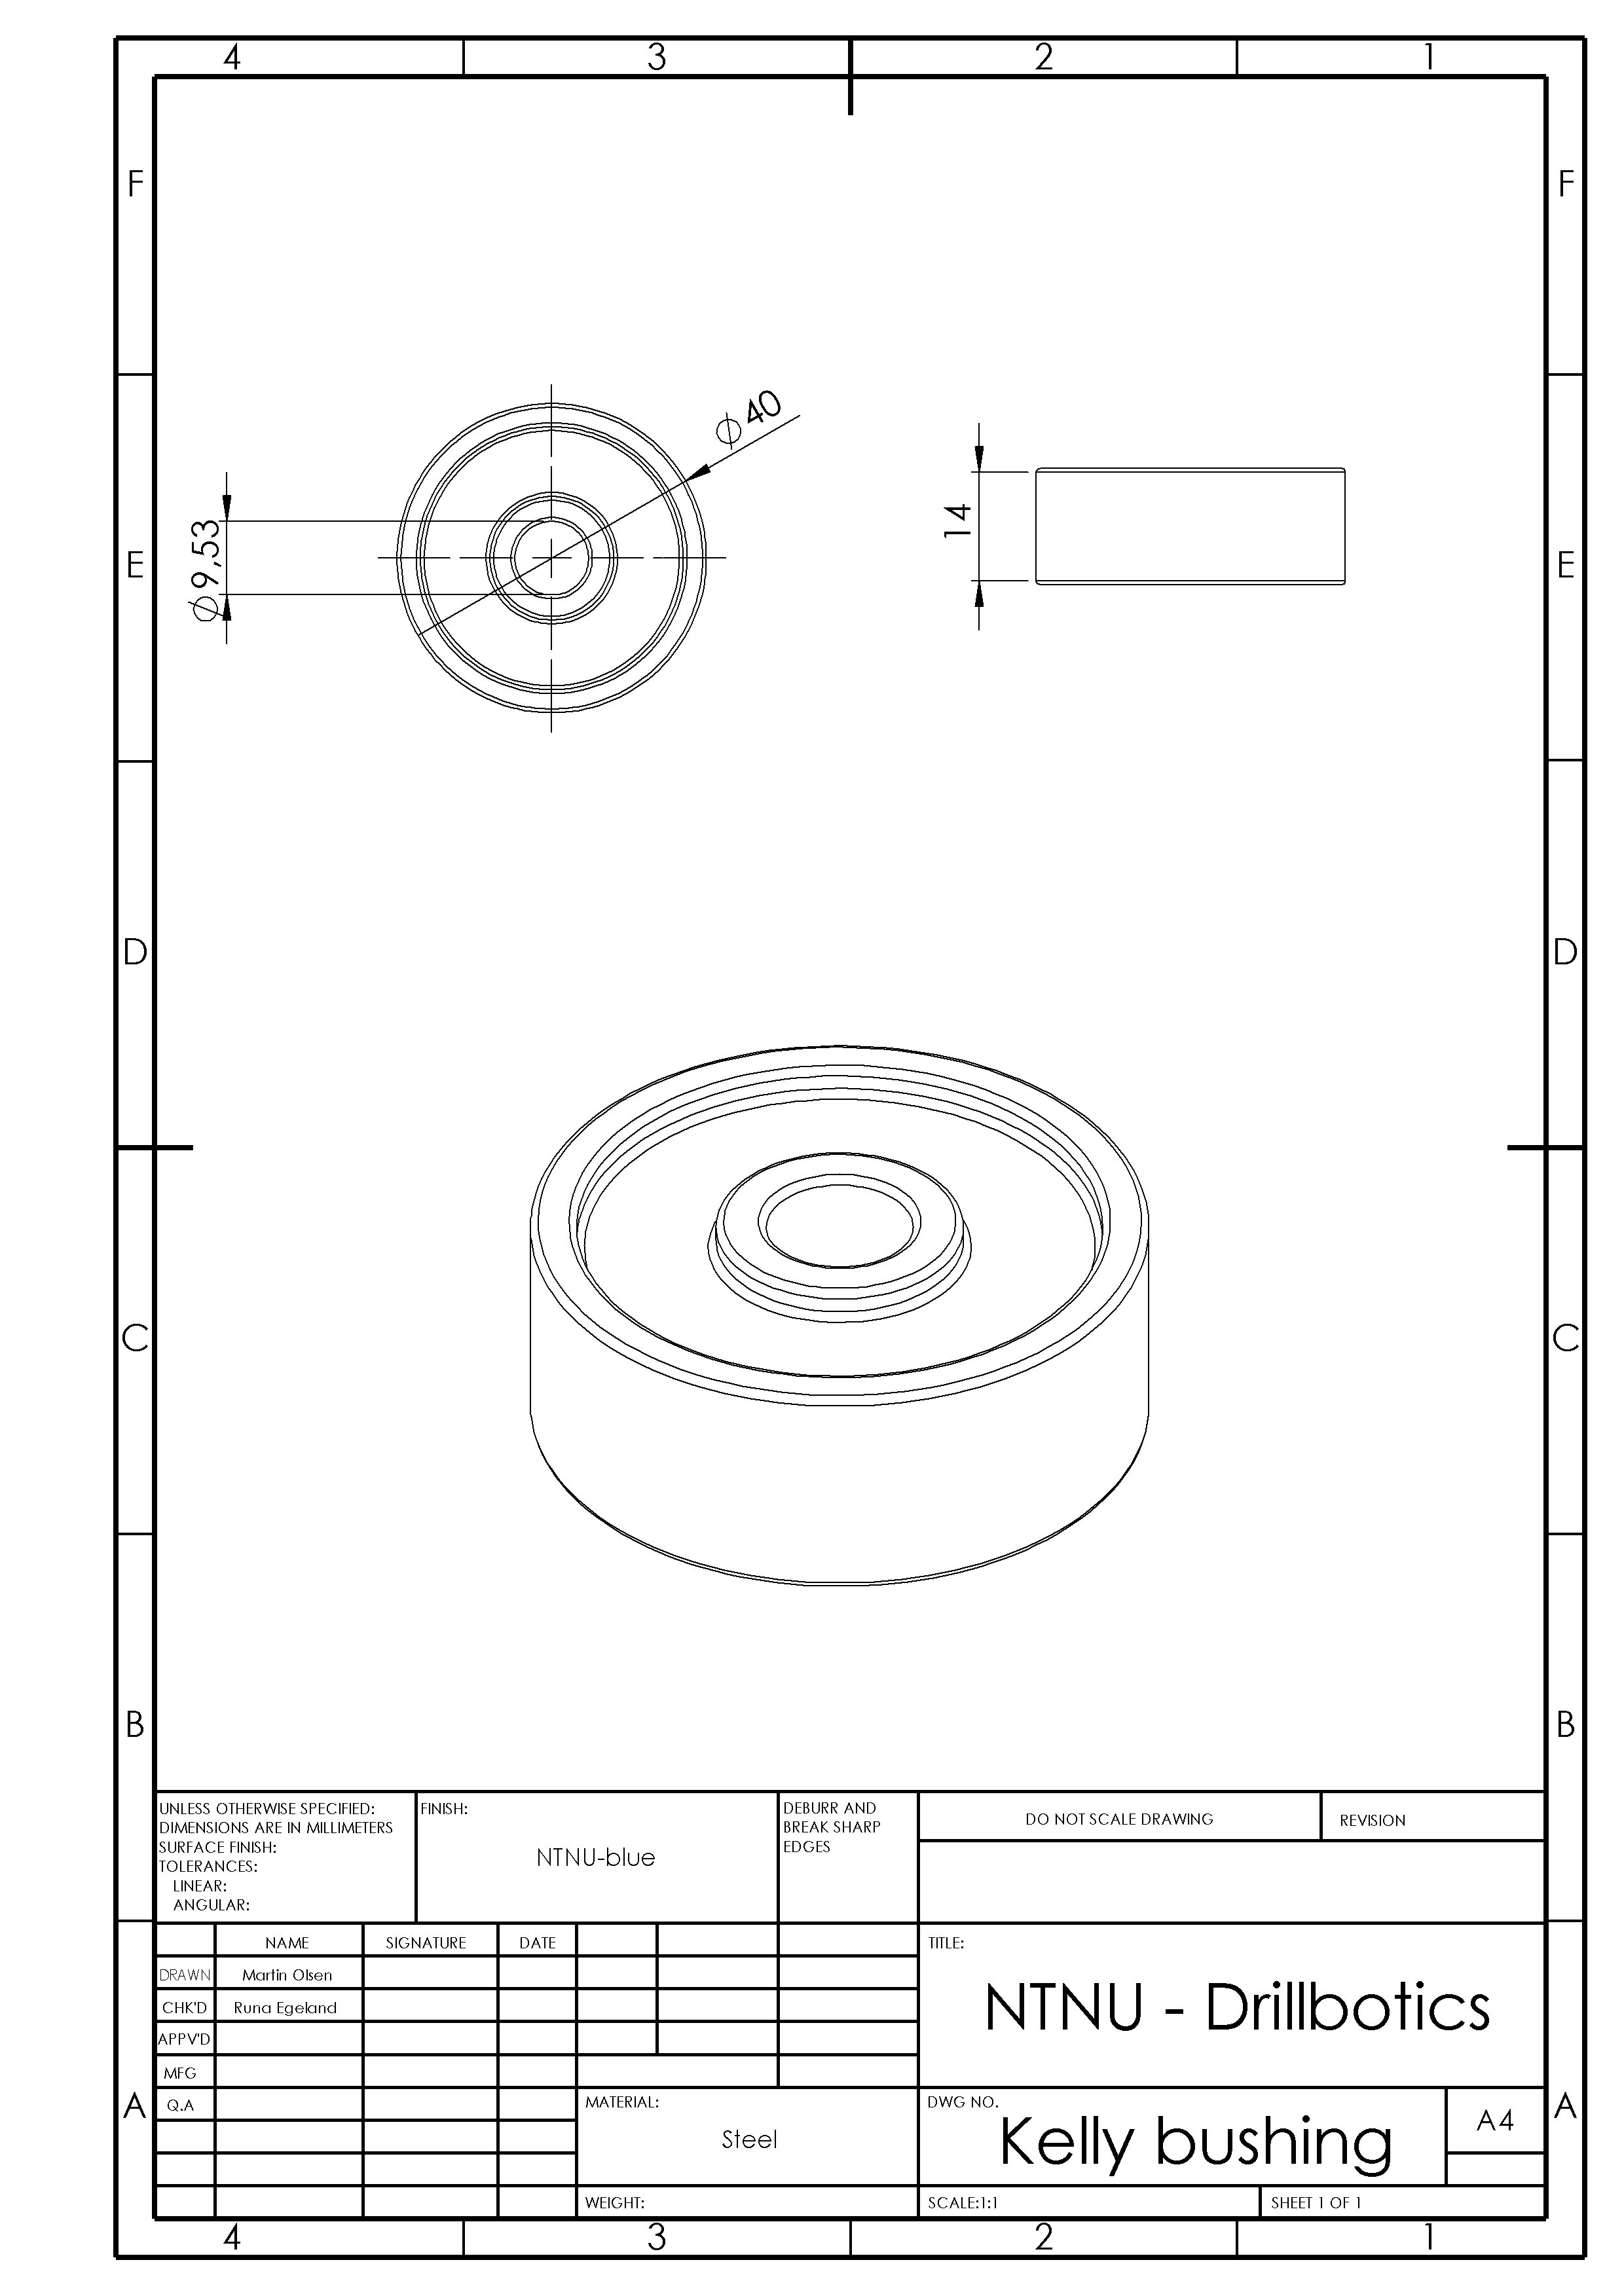
\includegraphics[width=1.0\textwidth]{figures/mechdrawings/Kellybushing.JPG}
\caption{Bushing for drilldeck. All dimensions in mm} 
\label{fig:bushing}
\end{figure}

\newpage
\begin{figure} [H]
\centering
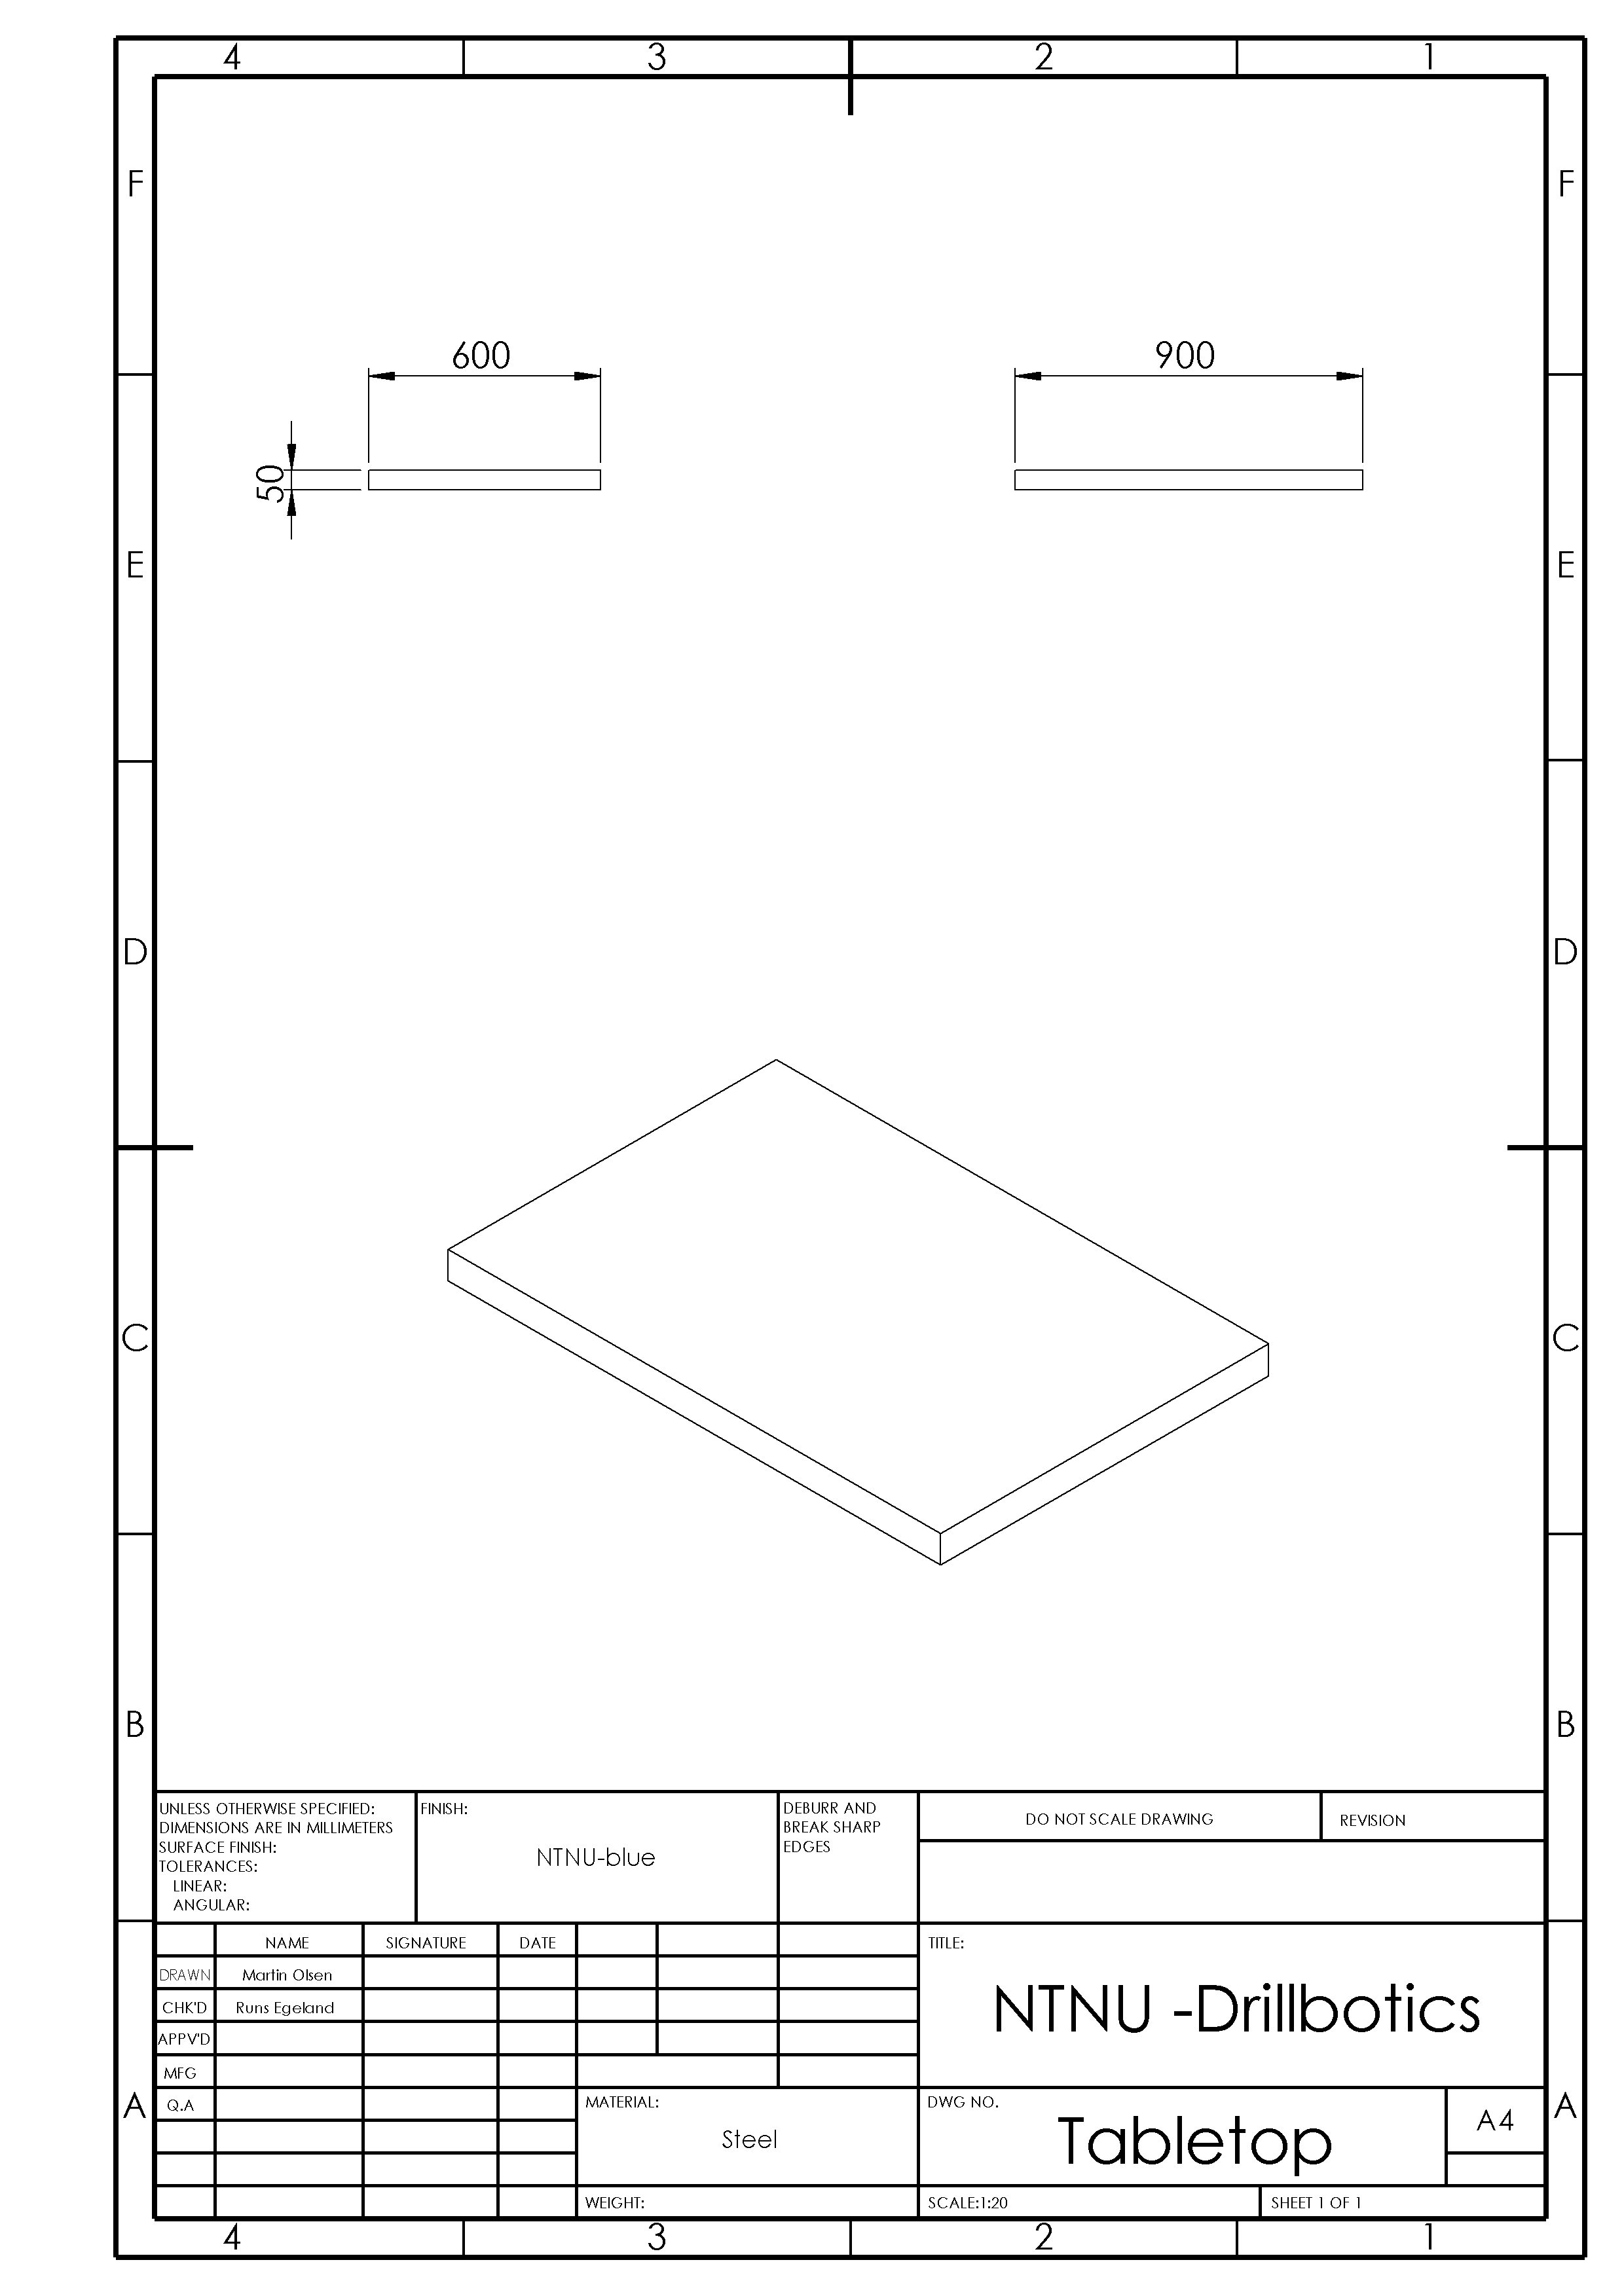
\includegraphics[width=1.0\textwidth]{figures/mechdrawings/Tabletop.JPG}
\caption{Tabletop. All dimensions in mm} 
\label{fig:tabletop}
\end{figure}

\newpage
\begin{figure} [H]
\centering
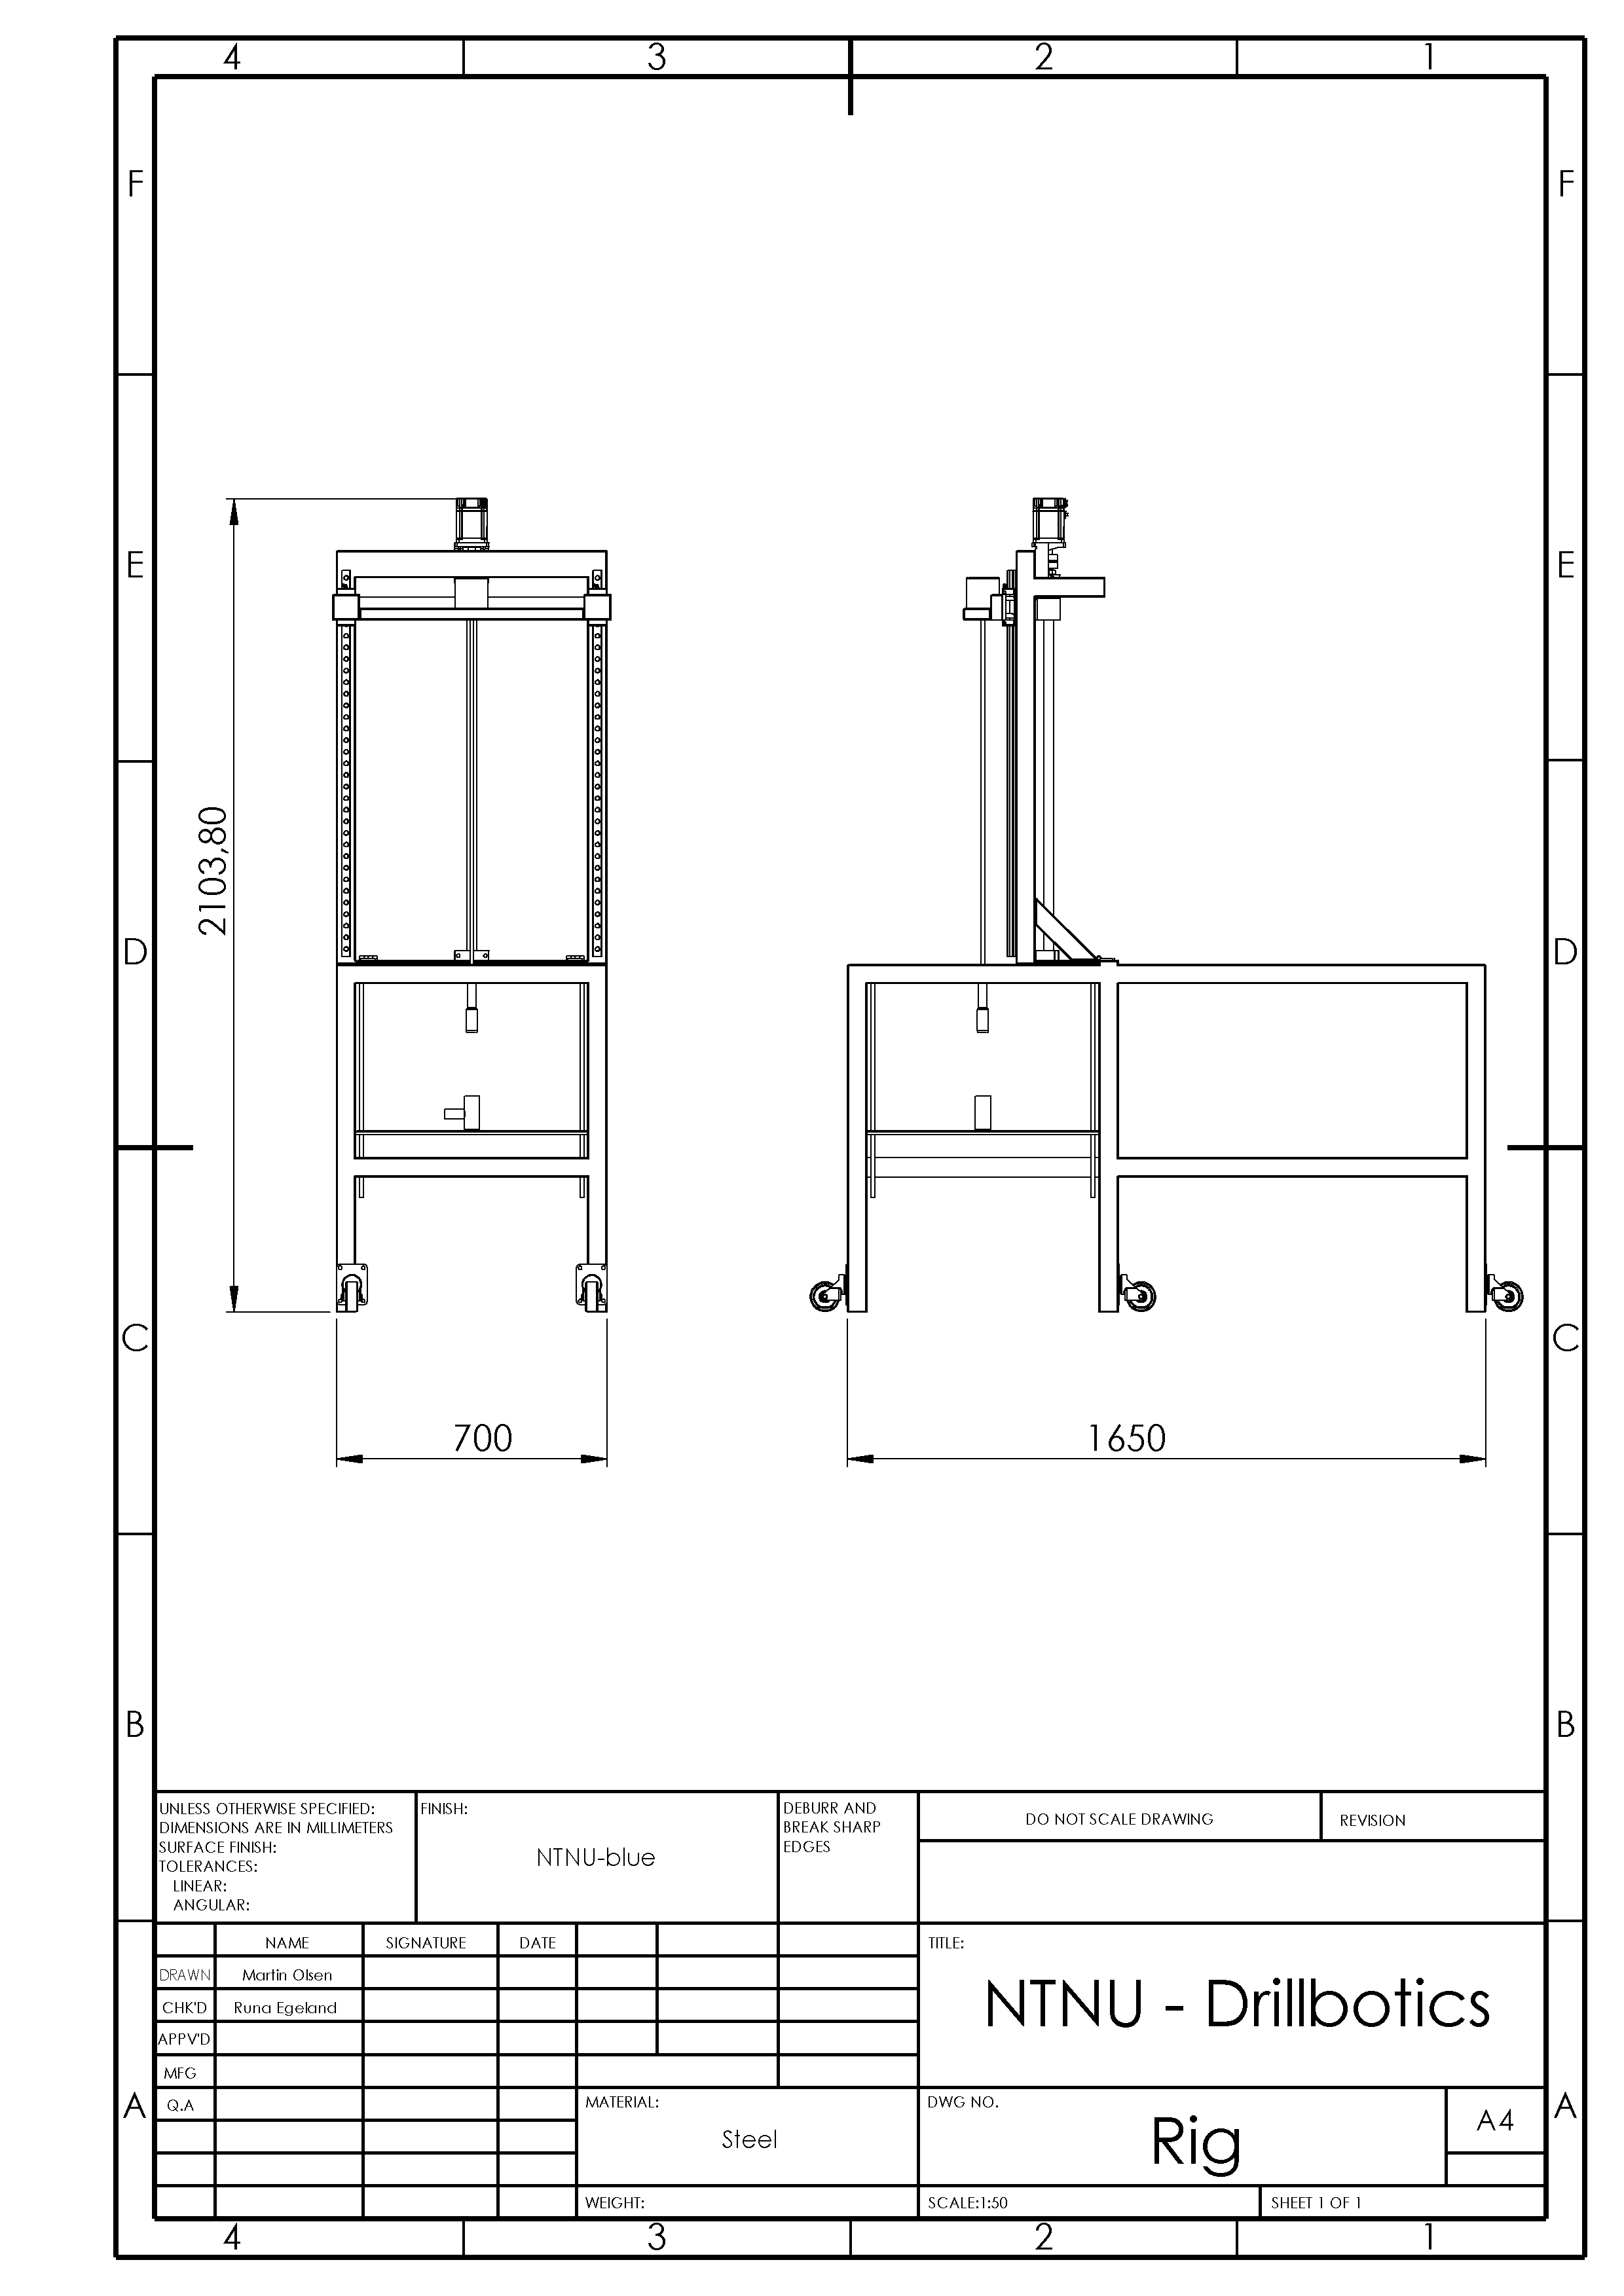
\includegraphics[width=1.0\textwidth]{figures/mechdrawings/Rigfrontandside.JPG}
\caption{Rig viewed from front and side. All dimensions in mm} 
\label{fig:rigview}
\end{figure}

\newpage
\begin{figure} [H]
\centering
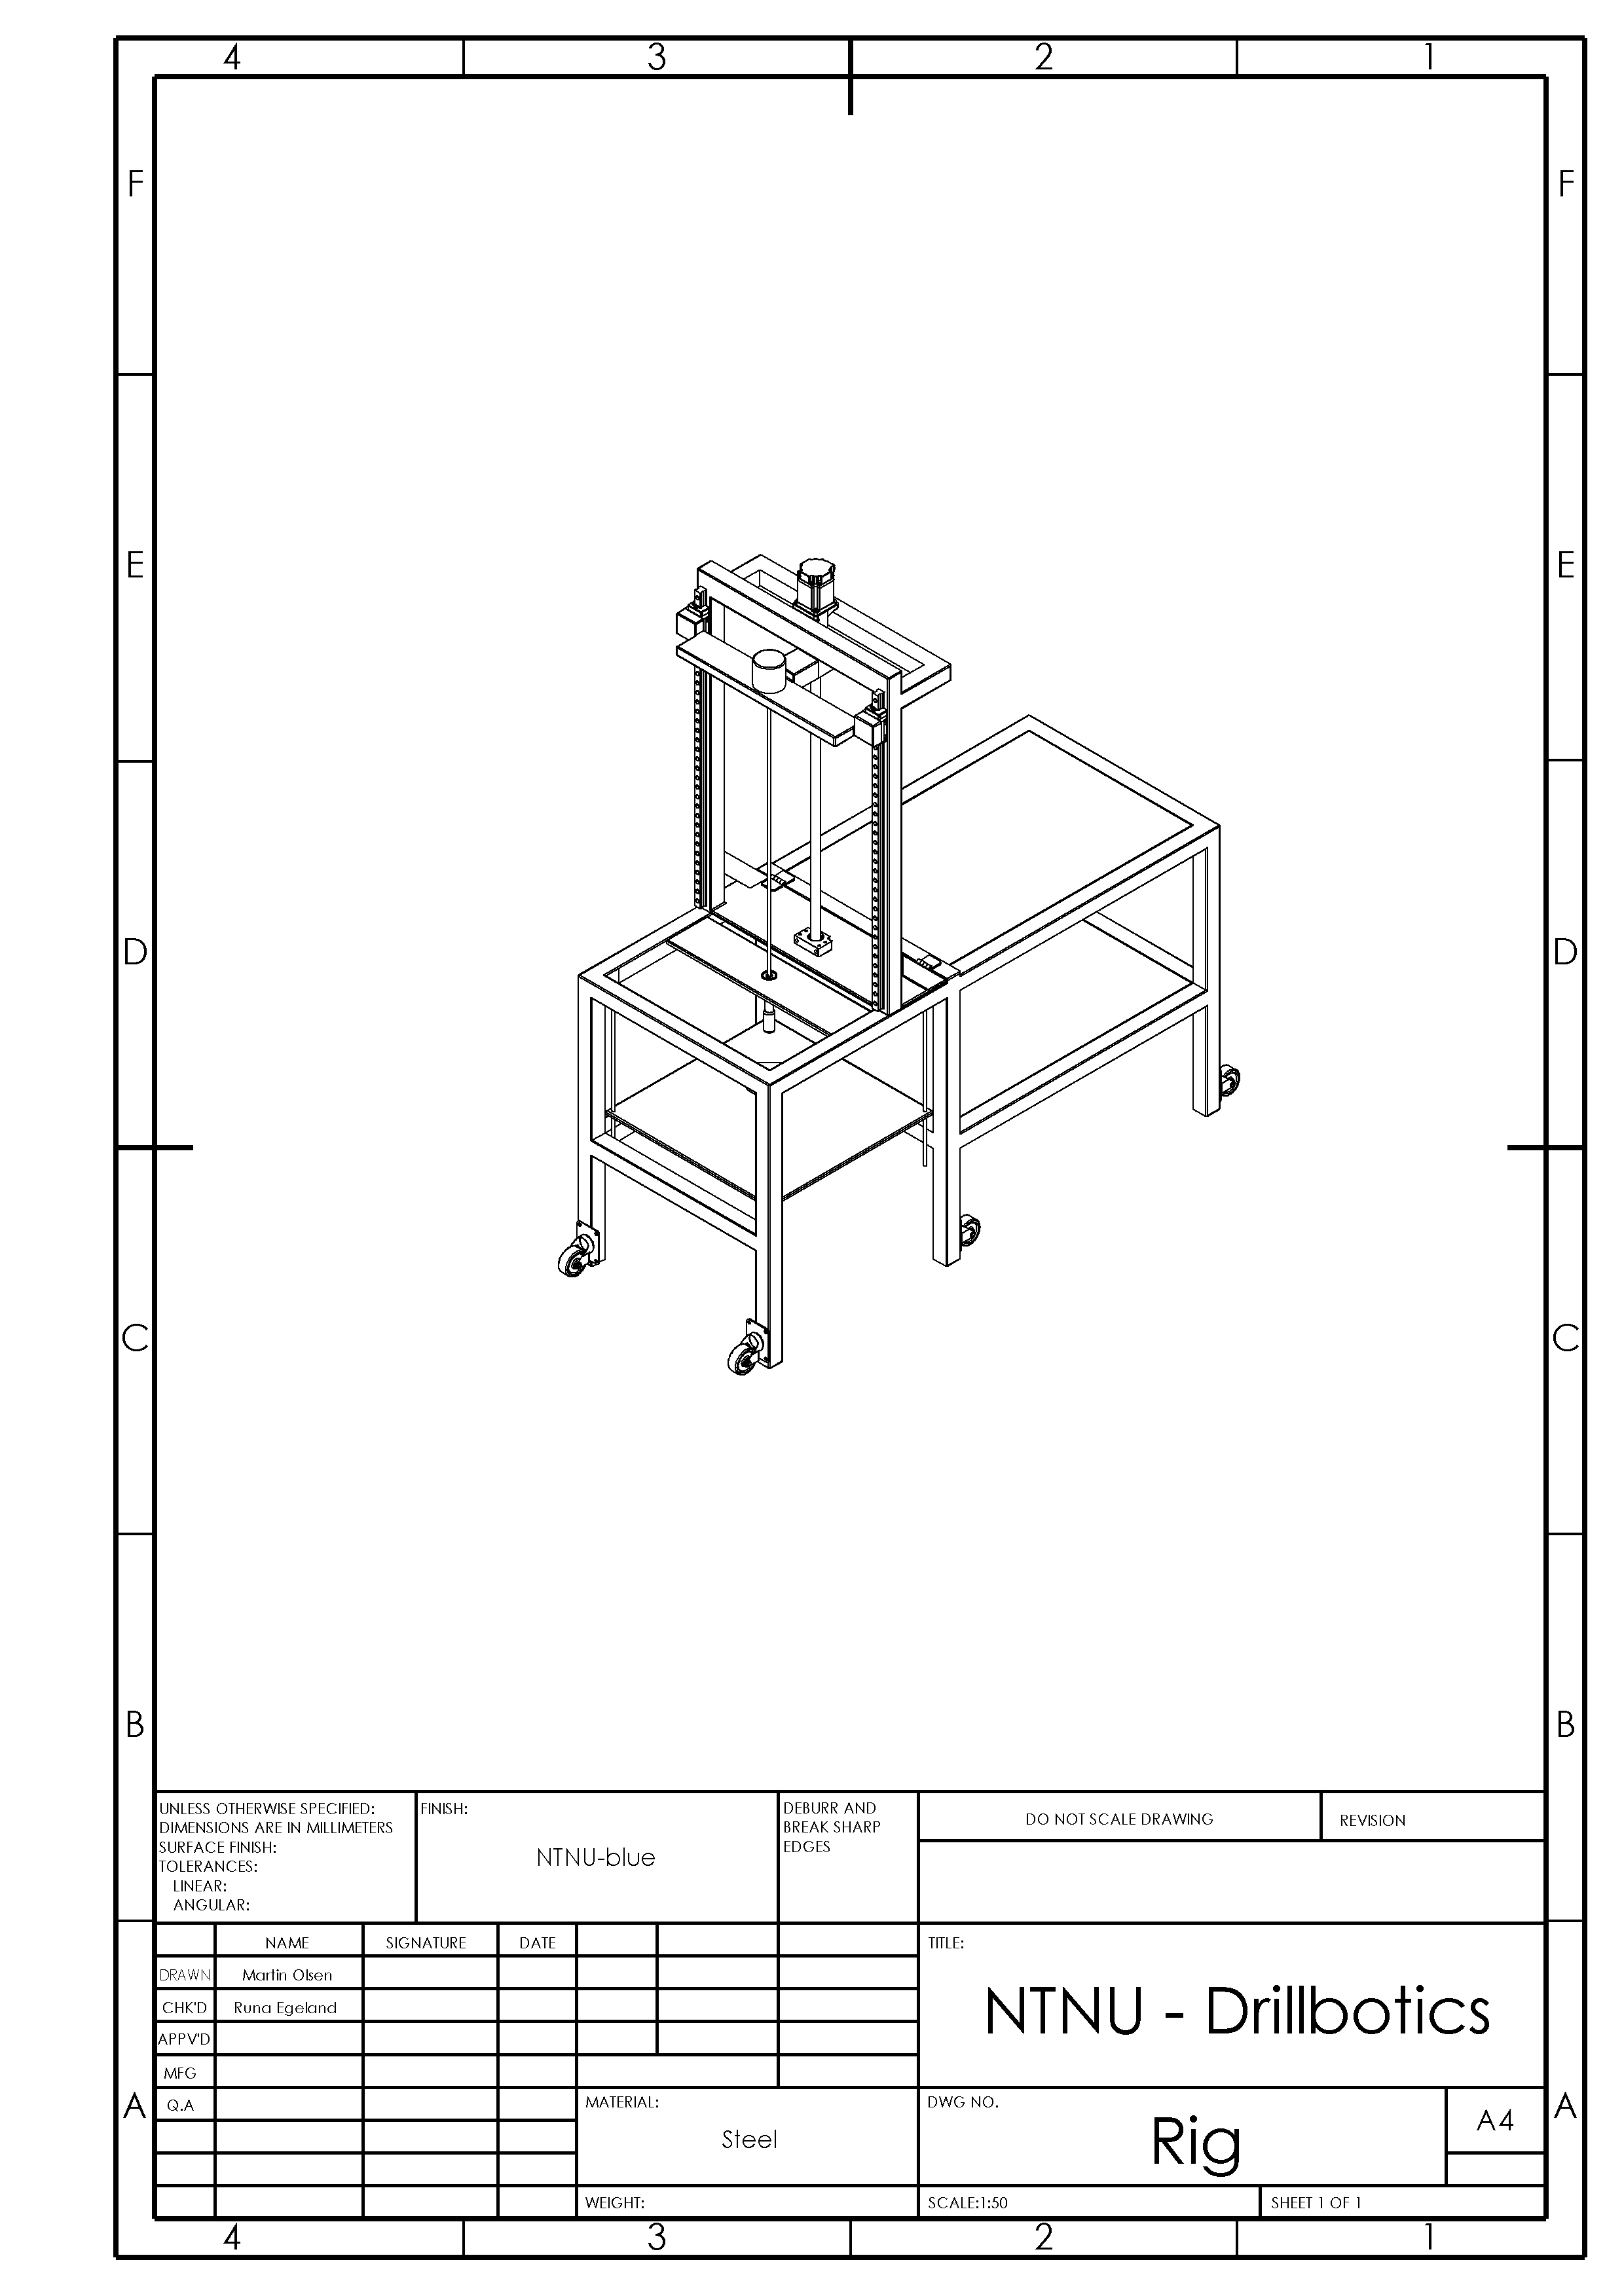
\includegraphics[width=1.0\textwidth]{figures/mechdrawings/Rig.JPG}
\caption{Assembled rig.} 
\label{fig:assemrig}
\end{figure}




\newpage
\section{Title of Appendix B} \label{App:AppendixB}


